\documentclass{article}
\usepackage[utf8]{inputenc}
\usepackage{geometry}
\usepackage{hyperref}
\usepackage{booktabs}
\usepackage{xcolor}
\usepackage{tikz}
\usetikzlibrary{positioning,arrows.meta}
\geometry{margin=1in}

\title{EPLE Algorithmic Elaboration Analysis Report}
\date{2025-09-15 17:39:18}
\author{EPLE Automated Analysis System}

\begin{document}
\maketitle

\section{Overview}

\textbf{Computational Patterns Detected:} 2\\
\textbf{Algorithmic Elaborations Found:} 16\\
\textbf{MUD Diagrams Generated:} 19\\

\section{Computational Patterns}

\begin{tabular}{@{}lll@{}}
\toprule
\textbf{Pattern} & \textbf{Type} & \textbf{Usage Count} \\
\midrule
base\_decomposition & decomposition & 4 \\
incremental\_counting & counting & 5 \\
\bottomrule
\end{tabular}

\section{Key Algorithmic Elaborations}

\begin{tabular}{@{}llll@{}}
\toprule
\textbf{Base Strategy} & \textbf{Elaborated Strategy} & \textbf{Shared Patterns} & \textbf{Confidence} \\
\midrule
ADD\_Rounding & SUB\_Rounding & base\_decomposition & 1.00 \\
ADD\_Rounding & SMR\_DIV\_CGOB & base\_decomposition & 1.00 \\
ADD\_Rounding & SMR\_DIV\_DealingByOnes & base\_decomposition & 1.00 \\
ADD\_Counting & ADD\_Chunking & incremental\_counting & 1.00 \\
ADD\_Counting & ADD\_COBO & incremental\_counting & 1.00 \\
ADD\_Counting & COBO & incremental\_counting & 1.00 \\
ADD\_Counting & SMR\_MULT\_C2C & incremental\_counting & 1.00 \\
ADD\_Chunking & ADD\_COBO & incremental\_counting & 1.00 \\
ADD\_Chunking & COBO & incremental\_counting & 1.00 \\
ADD\_Chunking & SMR\_MULT\_C2C & incremental\_counting & 1.00 \\
\bottomrule
\end{tabular}

\section{Meaning-Use Diagrams}

The following diagrams illustrate the algorithmic elaborations detected in the analysis.
Each diagram shows strategies connected by shared computational patterns.

\subsection{Addition To General}

\textbf{Operation:} Addition To General\\
\textbf{Strategies Analyzed:} 7\\
\textbf{Elaborations Detected:} 6\\

\begin{center}
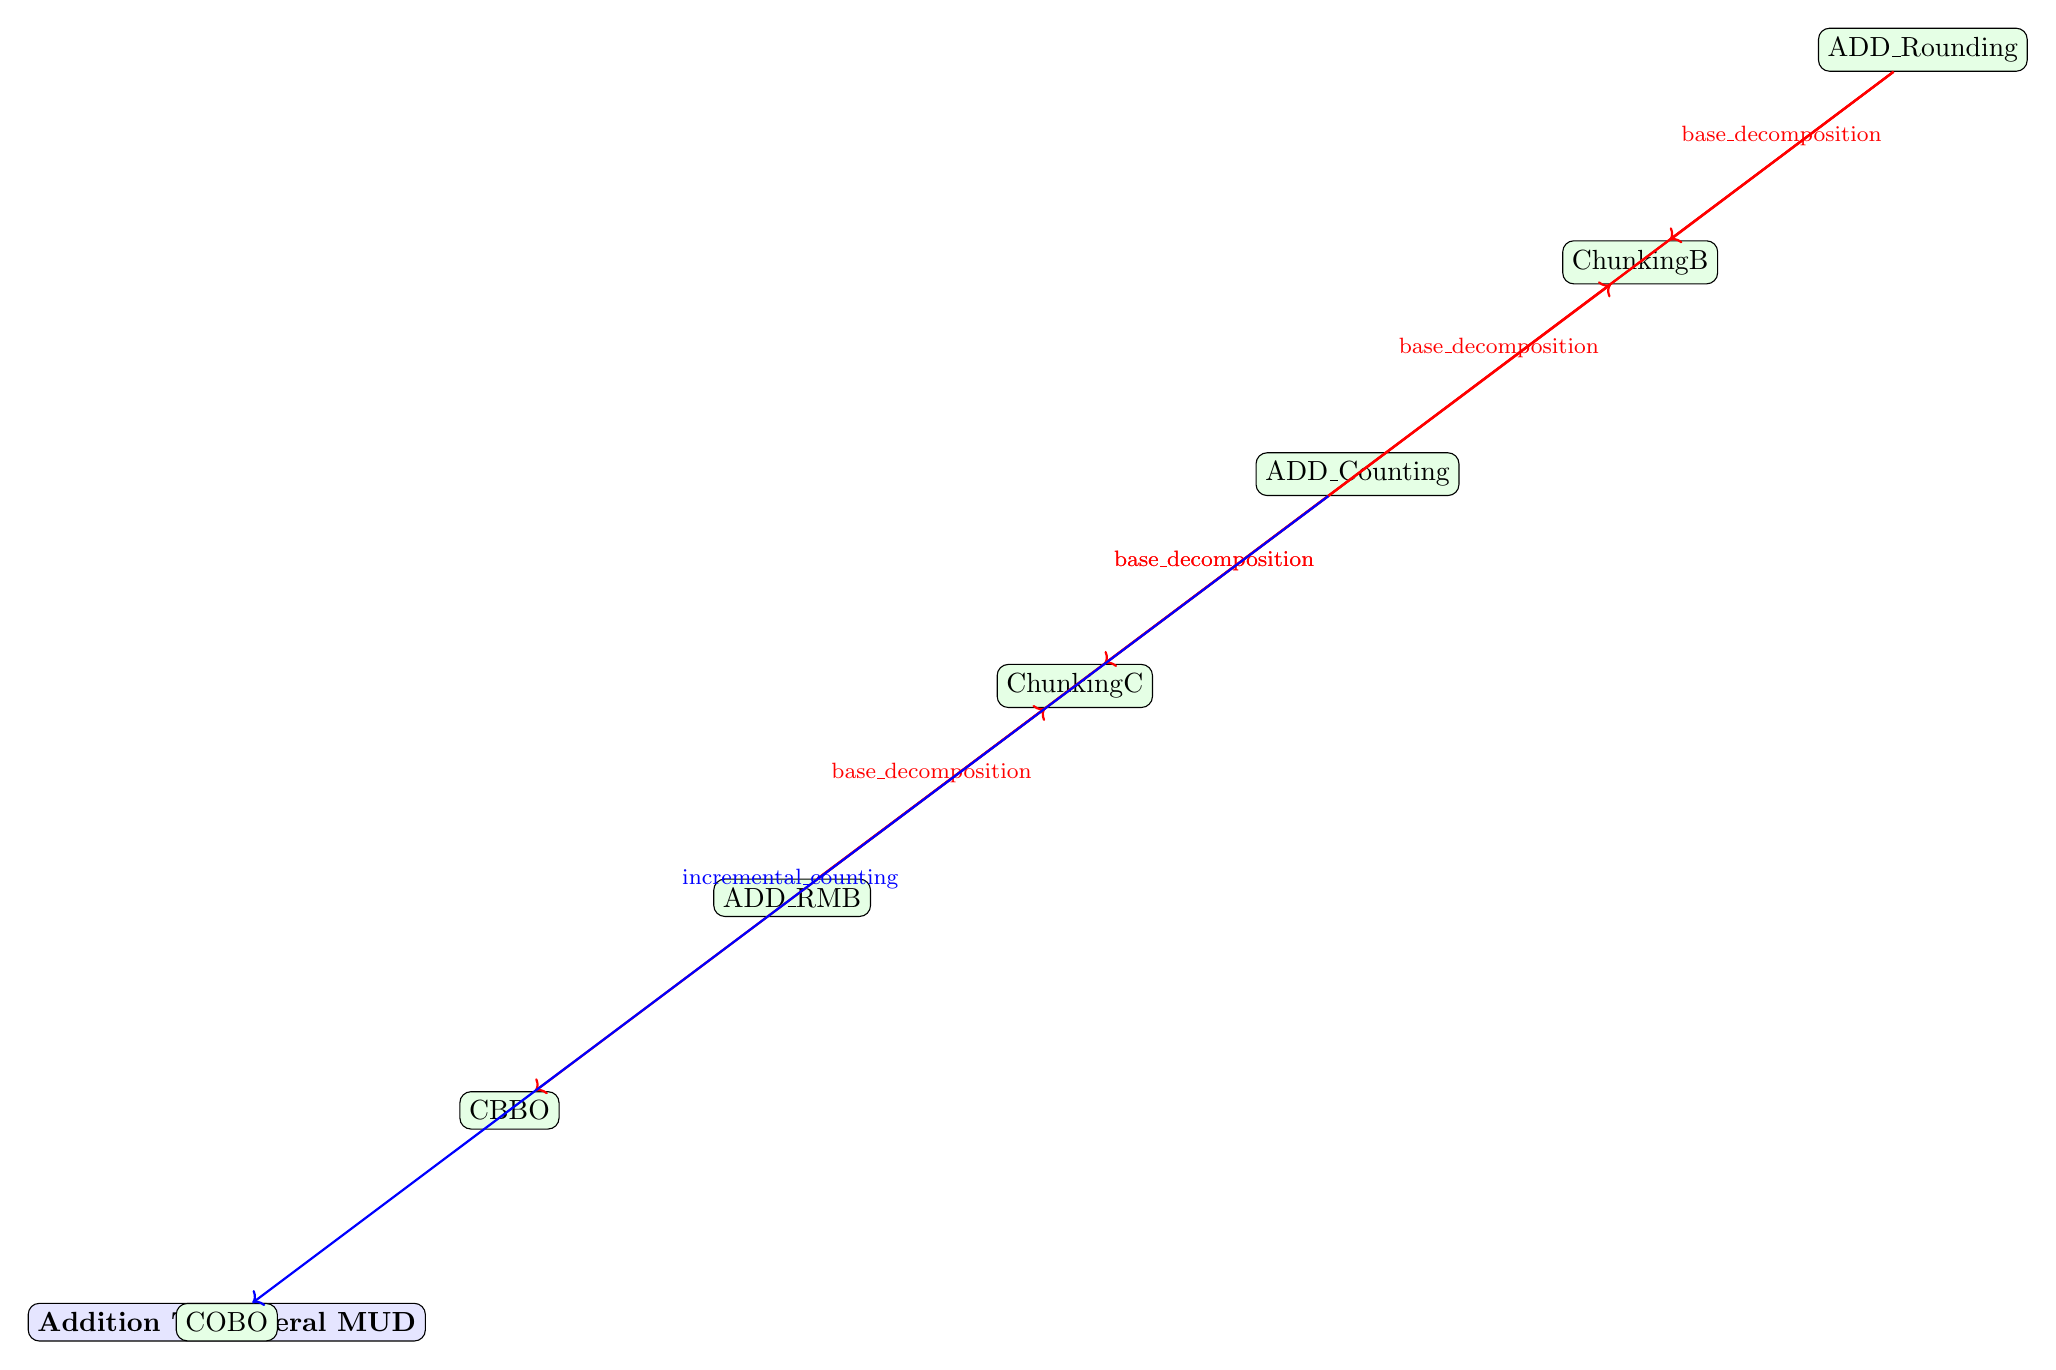
\begin{tikzpicture}[node distance=2cm and 2cm, auto]
\node[draw, fill=blue!10, rounded corners] (title) at (0,0) {\textbf{Addition To General MUD}};

\node[draw, fill=green!10, rounded corners] (strategy_0) at (0.00,0.00) {COBO};
\node[draw, fill=green!10, rounded corners] (strategy_1) at (3.59,2.69) {CBBO};
\node[draw, fill=green!10, rounded corners] (strategy_2) at (7.18,5.39) {ADD\_RMB};
\node[draw, fill=green!10, rounded corners] (strategy_3) at (10.77,8.08) {ChunkingC};
\node[draw, fill=green!10, rounded corners] (strategy_4) at (14.36,10.77) {ADD\_Counting};
\node[draw, fill=green!10, rounded corners] (strategy_5) at (17.95,13.46) {ChunkingB};
\node[draw, fill=green!10, rounded corners] (strategy_6) at (21.54,16.16) {ADD\_Rounding};

\draw[red, ->, thick] (strategy_6) -- (strategy_1)
    node[midway, above, font=\footnotesize] {base\_decomposition};
\draw[red, ->, thick] (strategy_6) -- (strategy_3)
    node[midway, above, font=\footnotesize] {base\_decomposition};
\draw[red, ->, thick] (strategy_6) -- (strategy_5)
    node[midway, above, font=\footnotesize] {base\_decomposition};
\draw[red, ->, thick] (strategy_2) -- (strategy_3)
    node[midway, above, font=\footnotesize] {base\_decomposition};
\draw[red, ->, thick] (strategy_2) -- (strategy_5)
    node[midway, above, font=\footnotesize] {base\_decomposition};
\draw[blue, ->, thick] (strategy_4) -- (strategy_0)
    node[midway, above, font=\footnotesize] {incremental\_counting};

\end{tikzpicture}
\end{center}

\textbf{Summary:}\\
\begin{verbatim}
Automated MUD Analysis for Addition To General
============================================================
Total strategies analyzed: 7
Total elaborations detected: 6

Key Patterns Identified:
  • base_decomposition: 5 relationships
  • incremental_counting: 1 relationships

Notable Elaborations:
  • ADD_Rounding → CBBO
    Shared: base_decomposition (confidence: 1.00)
  • ADD_Rounding → ChunkingC
    Shared: base_decomposition (confidence: 1.00)
  • ADD_Rounding → ChunkingB
    Shared: base_decomposition (confidence: 1.00)
  • ADD_Counting → COBO
    Shared: incremental_counting (confidence: 1.00)
  • ADD_RMB → ChunkingC
    Shared: base_decomposition (confidence: 1.00)
  ... and 1 more high-confidence relationships
\end{verbatim}

\newpage
\subsection{Addition}

\textbf{Operation:} Addition\\
\textbf{Strategies Analyzed:} 5\\
\textbf{Elaborations Detected:} 8\\

\begin{center}
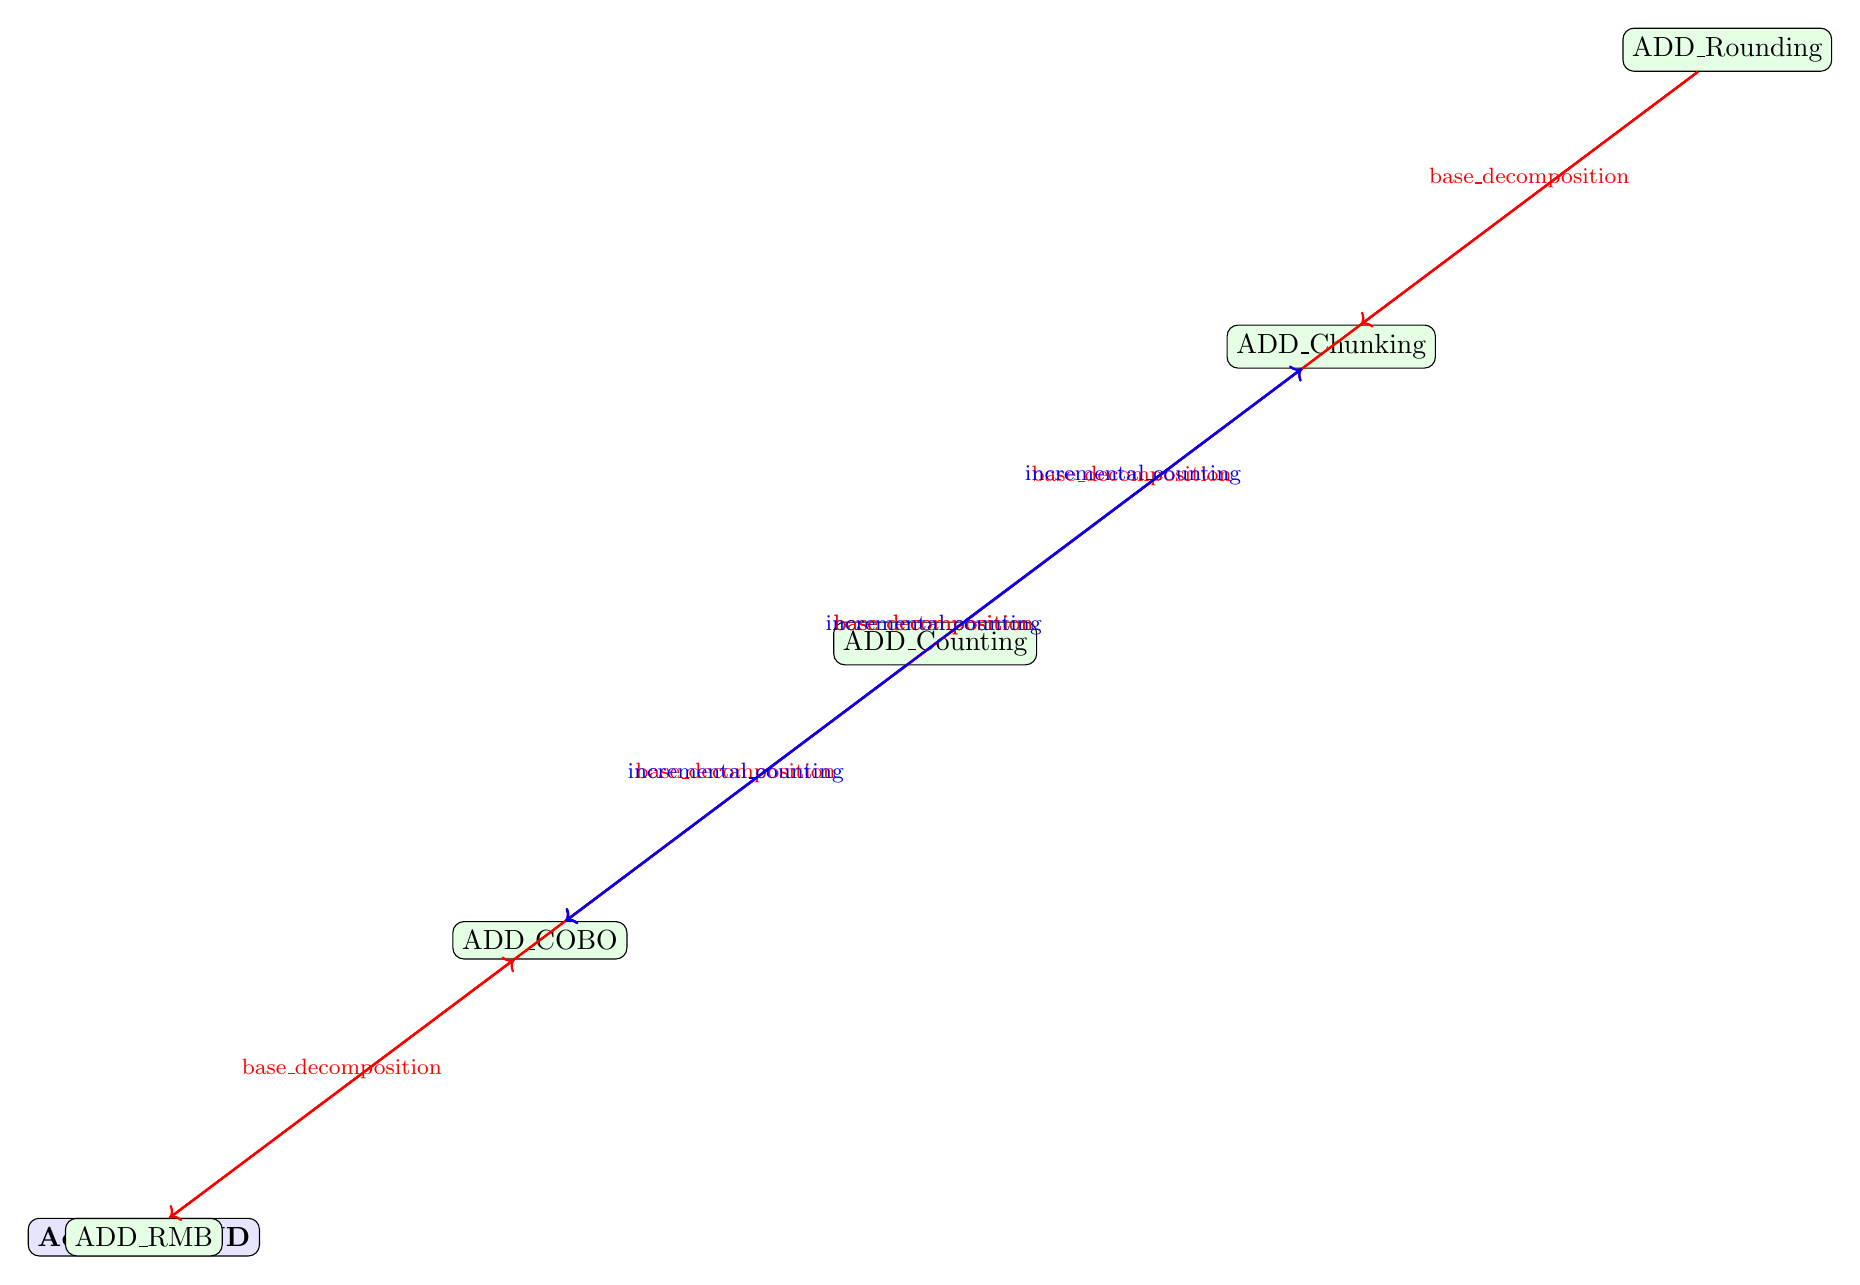
\begin{tikzpicture}[node distance=2cm and 2cm, auto]
\node[draw, fill=blue!10, rounded corners] (title) at (0,0) {\textbf{Addition MUD}};

\node[draw, fill=green!10, rounded corners] (strategy_0) at (0.00,0.00) {ADD\_RMB};
\node[draw, fill=green!10, rounded corners] (strategy_1) at (5.03,3.77) {ADD\_COBO};
\node[draw, fill=green!10, rounded corners] (strategy_2) at (10.05,7.54) {ADD\_Counting};
\node[draw, fill=green!10, rounded corners] (strategy_3) at (15.08,11.31) {ADD\_Chunking};
\node[draw, fill=green!10, rounded corners] (strategy_4) at (20.11,15.08) {ADD\_Rounding};

\draw[red, ->, thick] (strategy_4) -- (strategy_3)
    node[midway, above, font=\footnotesize] {base\_decomposition};
\draw[red, ->, thick] (strategy_4) -- (strategy_0)
    node[midway, above, font=\footnotesize] {base\_decomposition};
\draw[red, ->, thick] (strategy_4) -- (strategy_1)
    node[midway, above, font=\footnotesize] {base\_decomposition};
\draw[red, ->, thick] (strategy_0) -- (strategy_3)
    node[midway, above, font=\footnotesize] {base\_decomposition};
\draw[red, ->, thick] (strategy_3) -- (strategy_1)
    node[midway, above, font=\footnotesize] {base\_decomposition};
\draw[red, ->, thick] (strategy_0) -- (strategy_1)
    node[midway, above, font=\footnotesize] {base\_decomposition};
\draw[blue, ->, thick] (strategy_2) -- (strategy_3)
    node[midway, above, font=\footnotesize] {incremental\_counting};
\draw[blue, ->, thick] (strategy_2) -- (strategy_1)
    node[midway, above, font=\footnotesize] {incremental\_counting};
\draw[blue, ->, thick] (strategy_3) -- (strategy_1)
    node[midway, above, font=\footnotesize] {incremental\_counting};

\end{tikzpicture}
\end{center}

\textbf{Summary:}\\
\begin{verbatim}
Automated MUD Analysis for Addition
============================================================
Total strategies analyzed: 5
Total elaborations detected: 8

Key Patterns Identified:
  • base_decomposition: 6 relationships
  • incremental_counting: 3 relationships

Notable Elaborations:
  • ADD_Rounding → ADD_RMB
    Shared: base_decomposition (confidence: 1.00)
  • ADD_Chunking → ADD_COBO
    Shared: base_decomposition, incremental_counting (confidence: 1.00)
\end{verbatim}

\newpage
\subsection{Addition To Subtraction}

\textbf{Operation:} Addition To Subtraction\\
\textbf{Strategies Analyzed:} 5\\
\textbf{Elaborations Detected:} 6\\

\begin{center}
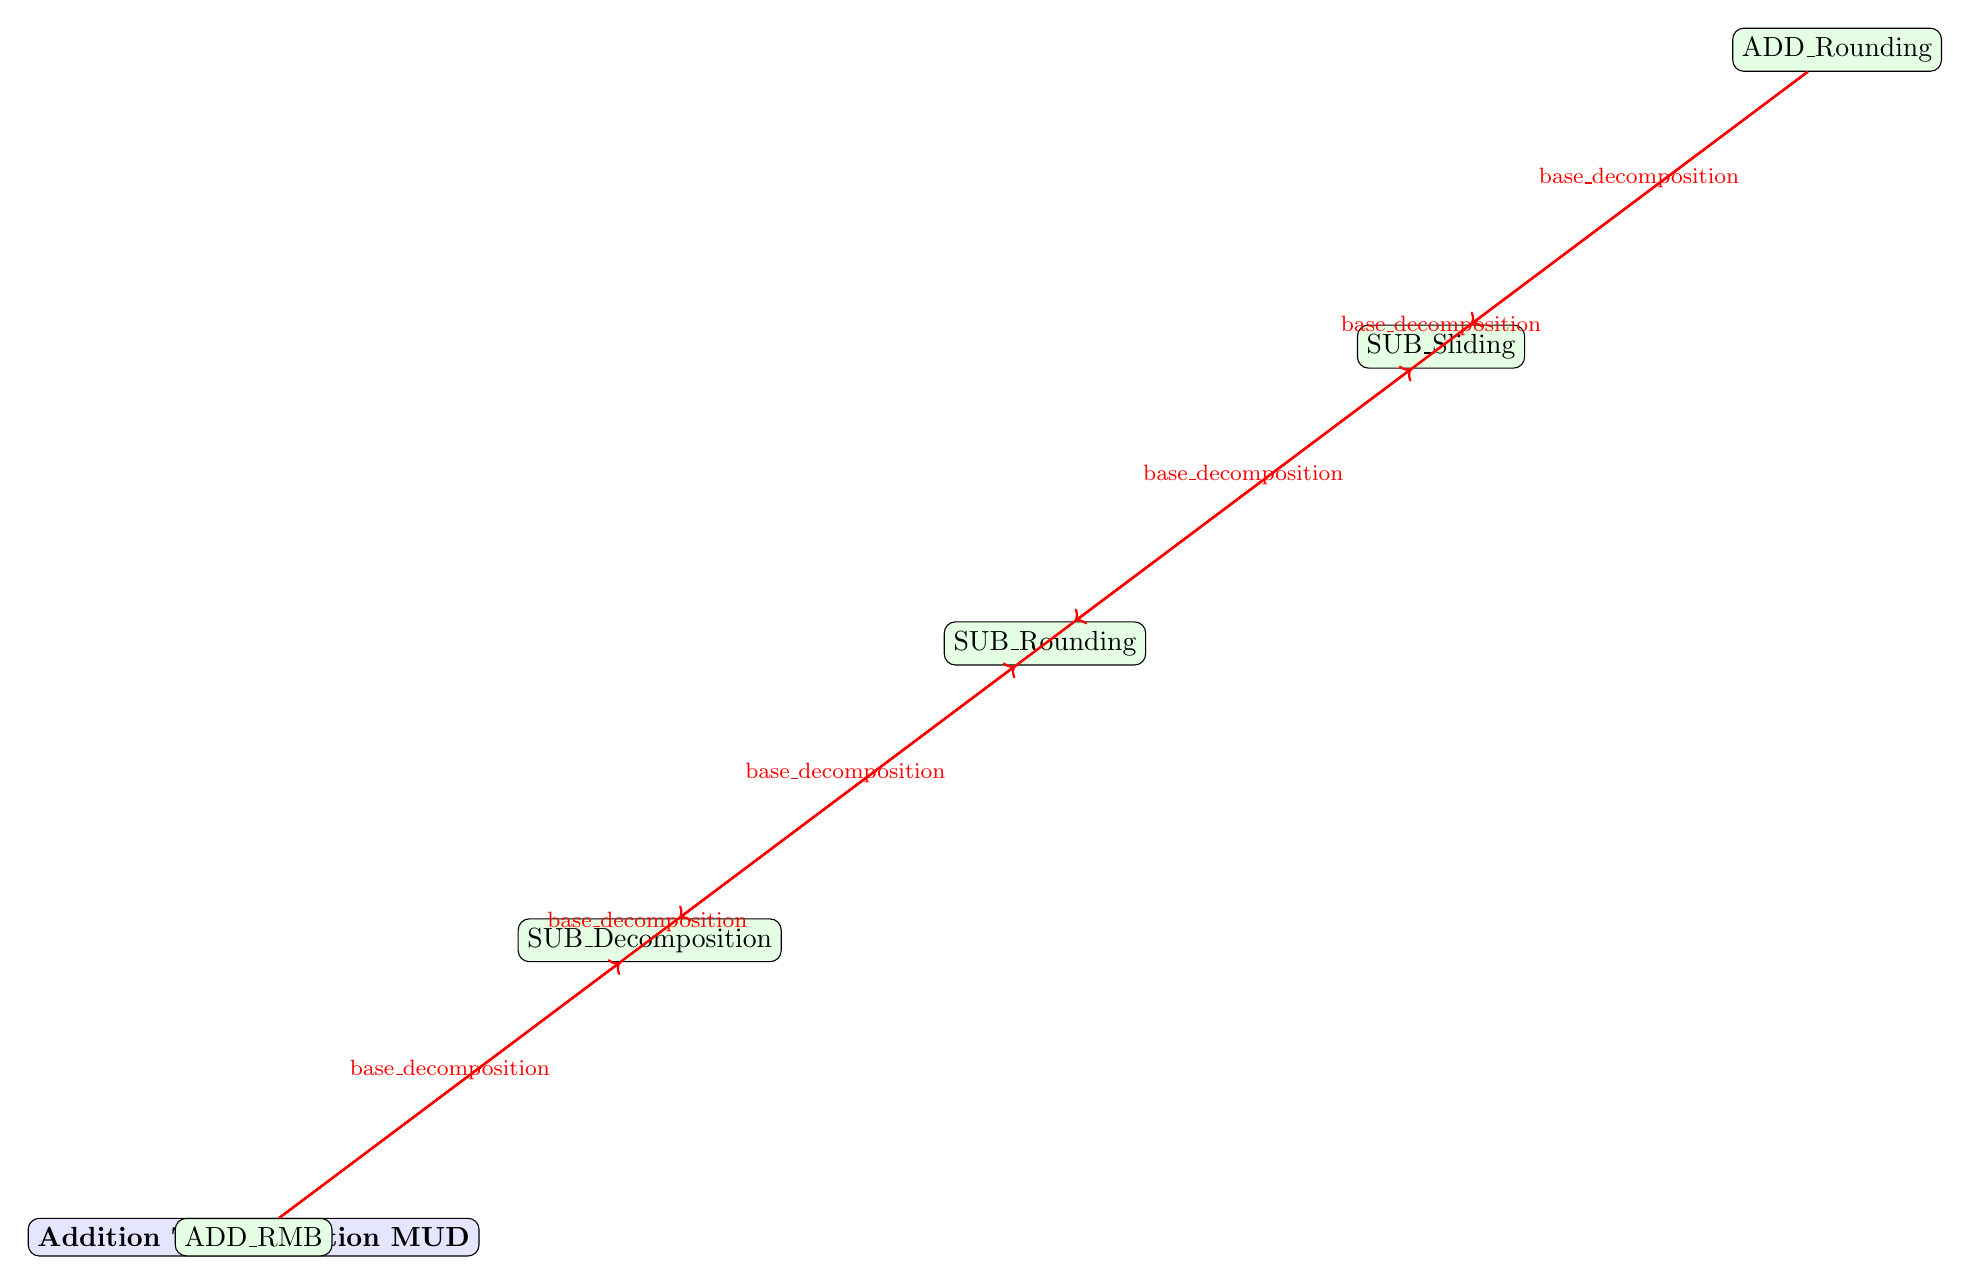
\begin{tikzpicture}[node distance=2cm and 2cm, auto]
\node[draw, fill=blue!10, rounded corners] (title) at (0,0) {\textbf{Addition To Subtraction MUD}};

\node[draw, fill=green!10, rounded corners] (strategy_0) at (0.00,0.00) {ADD\_RMB};
\node[draw, fill=green!10, rounded corners] (strategy_1) at (5.03,3.77) {SUB\_Decomposition};
\node[draw, fill=green!10, rounded corners] (strategy_2) at (10.05,7.54) {SUB\_Rounding};
\node[draw, fill=green!10, rounded corners] (strategy_3) at (15.08,11.31) {SUB\_Sliding};
\node[draw, fill=green!10, rounded corners] (strategy_4) at (20.11,15.08) {ADD\_Rounding};

\draw[red, ->, thick] (strategy_4) -- (strategy_3)
    node[midway, above, font=\footnotesize] {base\_decomposition};
\draw[red, ->, thick] (strategy_4) -- (strategy_1)
    node[midway, above, font=\footnotesize] {base\_decomposition};
\draw[red, ->, thick] (strategy_4) -- (strategy_2)
    node[midway, above, font=\footnotesize] {base\_decomposition};
\draw[red, ->, thick] (strategy_0) -- (strategy_3)
    node[midway, above, font=\footnotesize] {base\_decomposition};
\draw[red, ->, thick] (strategy_0) -- (strategy_1)
    node[midway, above, font=\footnotesize] {base\_decomposition};
\draw[red, ->, thick] (strategy_0) -- (strategy_2)
    node[midway, above, font=\footnotesize] {base\_decomposition};

\end{tikzpicture}
\end{center}

\textbf{Summary:}\\
\begin{verbatim}
Automated MUD Analysis for Addition To Subtraction
============================================================
Total strategies analyzed: 5
Total elaborations detected: 6

Key Patterns Identified:
  • base_decomposition: 6 relationships

Notable Elaborations:
  • ADD_Rounding → SUB_Sliding
    Shared: base_decomposition (confidence: 1.00)
  • ADD_Rounding → SUB_Decomposition
    Shared: base_decomposition (confidence: 1.00)
  • ADD_Rounding → SUB_Rounding
    Shared: base_decomposition (confidence: 1.00)
  • ADD_RMB → SUB_Sliding
    Shared: base_decomposition (confidence: 1.00)
  • ADD_RMB → SUB_Decomposition
    Shared: base_decomposition (confidence: 1.00)
  ... and 1 more high-confidence relationships
\end{verbatim}

\newpage
\subsection{Addition To Multiplication}

\textbf{Operation:} Addition To Multiplication\\
\textbf{Strategies Analyzed:} 5\\
\textbf{Elaborations Detected:} 3\\

\begin{center}
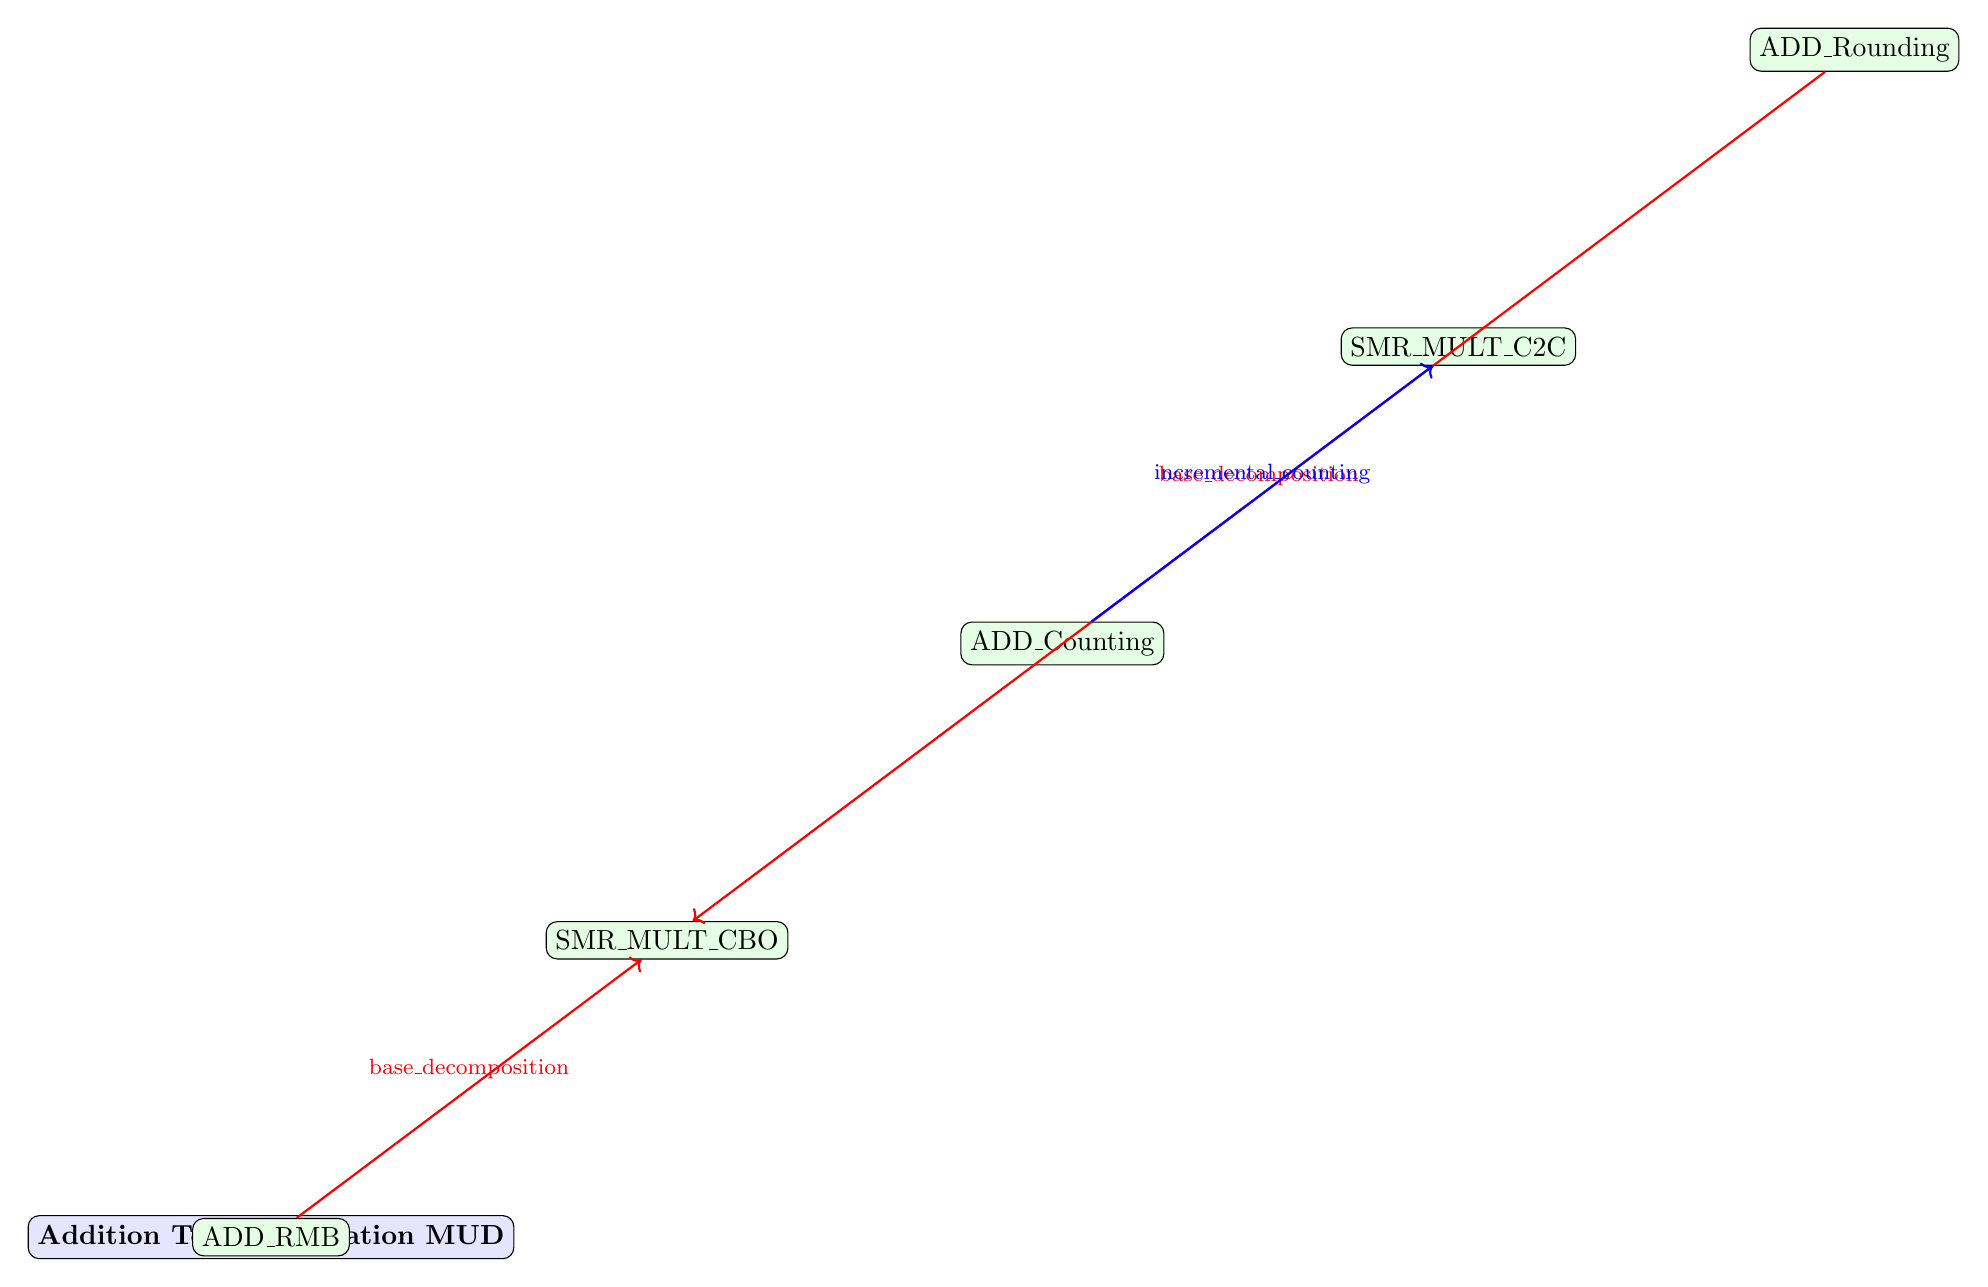
\begin{tikzpicture}[node distance=2cm and 2cm, auto]
\node[draw, fill=blue!10, rounded corners] (title) at (0,0) {\textbf{Addition To Multiplication MUD}};

\node[draw, fill=green!10, rounded corners] (strategy_0) at (0.00,0.00) {ADD\_RMB};
\node[draw, fill=green!10, rounded corners] (strategy_1) at (5.03,3.77) {SMR\_MULT\_CBO};
\node[draw, fill=green!10, rounded corners] (strategy_2) at (10.05,7.54) {ADD\_Counting};
\node[draw, fill=green!10, rounded corners] (strategy_3) at (15.08,11.31) {SMR\_MULT\_C2C};
\node[draw, fill=green!10, rounded corners] (strategy_4) at (20.11,15.08) {ADD\_Rounding};

\draw[red, ->, thick] (strategy_4) -- (strategy_1)
    node[midway, above, font=\footnotesize] {base\_decomposition};
\draw[red, ->, thick] (strategy_0) -- (strategy_1)
    node[midway, above, font=\footnotesize] {base\_decomposition};
\draw[blue, ->, thick] (strategy_2) -- (strategy_3)
    node[midway, above, font=\footnotesize] {incremental\_counting};

\end{tikzpicture}
\end{center}

\textbf{Summary:}\\
\begin{verbatim}
Automated MUD Analysis for Addition To Multiplication
============================================================
Total strategies analyzed: 5
Total elaborations detected: 3

Key Patterns Identified:
  • base_decomposition: 2 relationships
  • incremental_counting: 1 relationships

Notable Elaborations:
  • ADD_Rounding → SMR_MULT_CBO
    Shared: base_decomposition (confidence: 1.00)
  • ADD_Counting → SMR_MULT_C2C
    Shared: incremental_counting (confidence: 1.00)
  • ADD_RMB → SMR_MULT_CBO
    Shared: base_decomposition (confidence: 1.00)
\end{verbatim}

\newpage
\subsection{Addition To Division}

\textbf{Operation:} Addition To Division\\
\textbf{Strategies Analyzed:} 4\\
\textbf{Elaborations Detected:} 4\\

\begin{center}
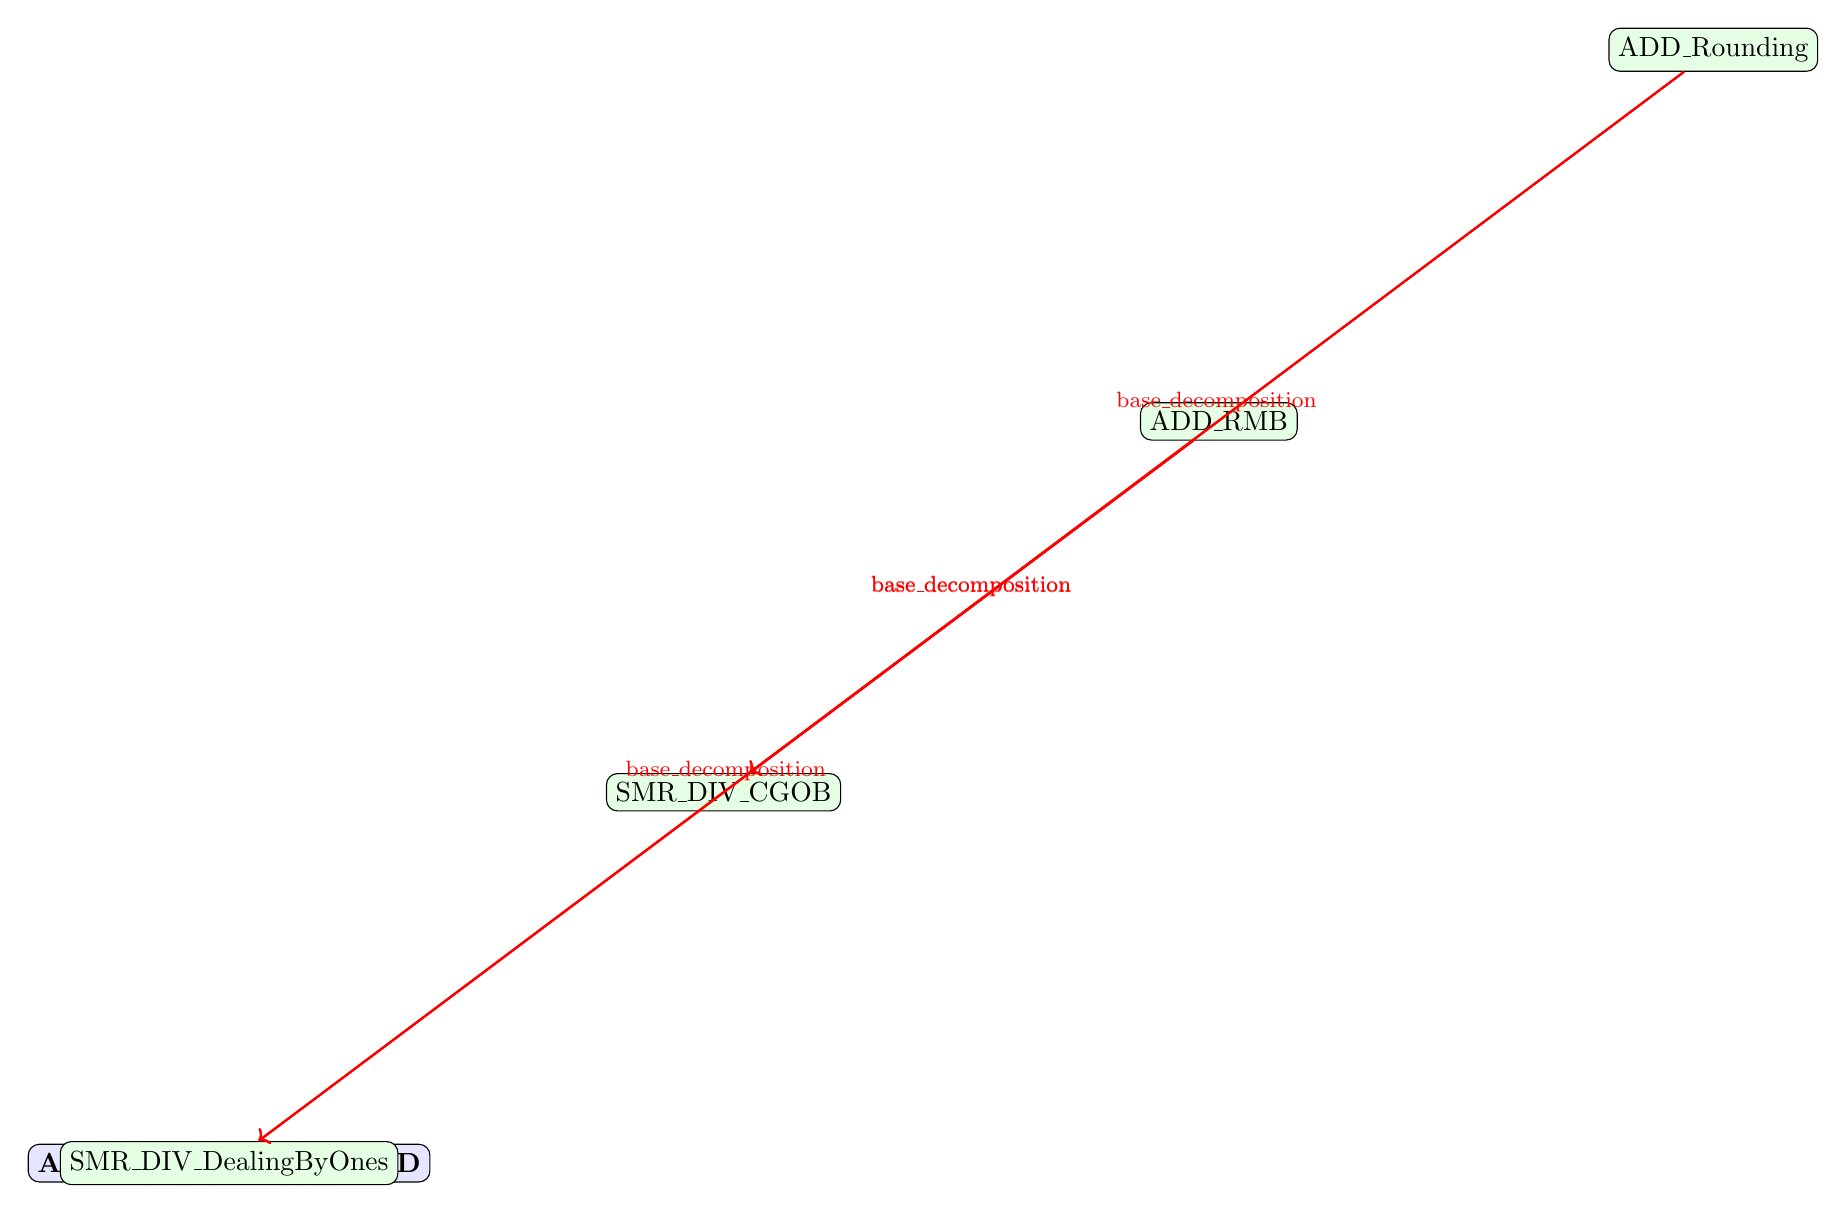
\begin{tikzpicture}[node distance=2cm and 2cm, auto]
\node[draw, fill=blue!10, rounded corners] (title) at (0,0) {\textbf{Addition To Division MUD}};

\node[draw, fill=green!10, rounded corners] (strategy_0) at (0.00,0.00) {SMR\_DIV\_DealingByOnes};
\node[draw, fill=green!10, rounded corners] (strategy_1) at (6.28,4.71) {SMR\_DIV\_CGOB};
\node[draw, fill=green!10, rounded corners] (strategy_2) at (12.57,9.42) {ADD\_RMB};
\node[draw, fill=green!10, rounded corners] (strategy_3) at (18.85,14.14) {ADD\_Rounding};

\draw[red, ->, thick] (strategy_3) -- (strategy_1)
    node[midway, above, font=\footnotesize] {base\_decomposition};
\draw[red, ->, thick] (strategy_3) -- (strategy_0)
    node[midway, above, font=\footnotesize] {base\_decomposition};
\draw[red, ->, thick] (strategy_2) -- (strategy_1)
    node[midway, above, font=\footnotesize] {base\_decomposition};
\draw[red, ->, thick] (strategy_2) -- (strategy_0)
    node[midway, above, font=\footnotesize] {base\_decomposition};

\end{tikzpicture}
\end{center}

\textbf{Summary:}\\
\begin{verbatim}
Automated MUD Analysis for Addition To Division
============================================================
Total strategies analyzed: 4
Total elaborations detected: 4

Key Patterns Identified:
  • base_decomposition: 4 relationships

Notable Elaborations:
  • ADD_Rounding → SMR_DIV_CGOB
    Shared: base_decomposition (confidence: 1.00)
  • ADD_Rounding → SMR_DIV_DealingByOnes
    Shared: base_decomposition (confidence: 1.00)
  • ADD_RMB → SMR_DIV_CGOB
    Shared: base_decomposition (confidence: 1.00)
  • ADD_RMB → SMR_DIV_DealingByOnes
    Shared: base_decomposition (confidence: 1.00)
\end{verbatim}

\newpage
\subsection{General To Addition}

\textbf{Operation:} General To Addition\\
\textbf{Strategies Analyzed:} 7\\
\textbf{Elaborations Detected:} 9\\

\begin{center}
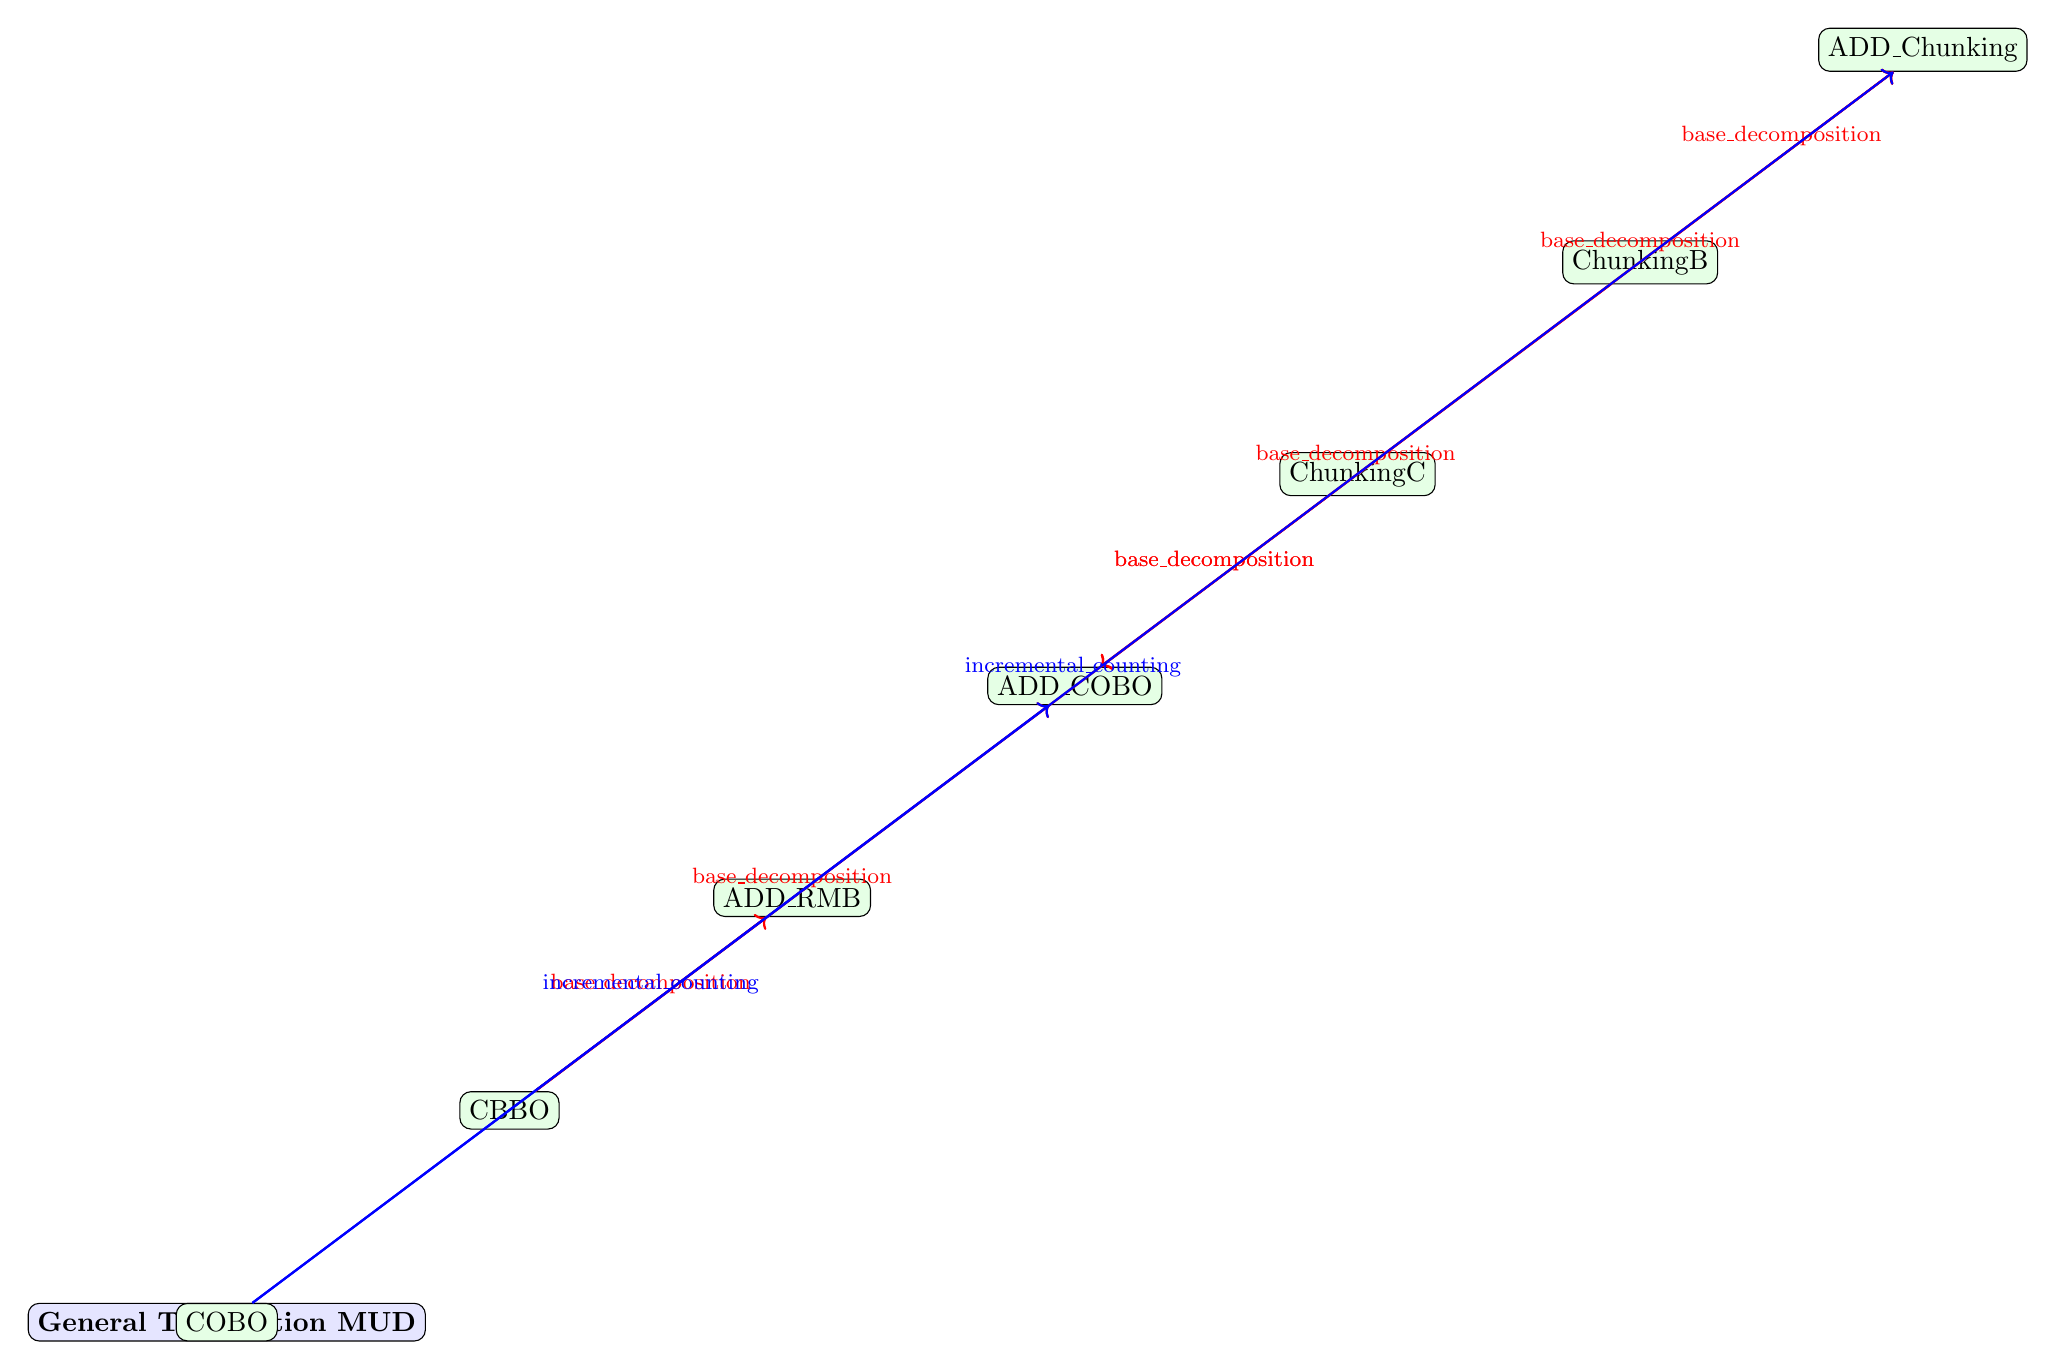
\begin{tikzpicture}[node distance=2cm and 2cm, auto]
\node[draw, fill=blue!10, rounded corners] (title) at (0,0) {\textbf{General To Addition MUD}};

\node[draw, fill=green!10, rounded corners] (strategy_0) at (0.00,0.00) {COBO};
\node[draw, fill=green!10, rounded corners] (strategy_1) at (3.59,2.69) {CBBO};
\node[draw, fill=green!10, rounded corners] (strategy_2) at (7.18,5.39) {ADD\_RMB};
\node[draw, fill=green!10, rounded corners] (strategy_3) at (10.77,8.08) {ADD\_COBO};
\node[draw, fill=green!10, rounded corners] (strategy_4) at (14.36,10.77) {ChunkingC};
\node[draw, fill=green!10, rounded corners] (strategy_5) at (17.95,13.46) {ChunkingB};
\node[draw, fill=green!10, rounded corners] (strategy_6) at (21.54,16.16) {ADD\_Chunking};

\draw[red, ->, thick] (strategy_1) -- (strategy_6)
    node[midway, above, font=\footnotesize] {base\_decomposition};
\draw[red, ->, thick] (strategy_1) -- (strategy_2)
    node[midway, above, font=\footnotesize] {base\_decomposition};
\draw[red, ->, thick] (strategy_1) -- (strategy_3)
    node[midway, above, font=\footnotesize] {base\_decomposition};
\draw[red, ->, thick] (strategy_4) -- (strategy_6)
    node[midway, above, font=\footnotesize] {base\_decomposition};
\draw[red, ->, thick] (strategy_5) -- (strategy_6)
    node[midway, above, font=\footnotesize] {base\_decomposition};
\draw[red, ->, thick] (strategy_4) -- (strategy_3)
    node[midway, above, font=\footnotesize] {base\_decomposition};
\draw[red, ->, thick] (strategy_5) -- (strategy_3)
    node[midway, above, font=\footnotesize] {base\_decomposition};
\draw[blue, ->, thick] (strategy_0) -- (strategy_6)
    node[midway, above, font=\footnotesize] {incremental\_counting};
\draw[blue, ->, thick] (strategy_0) -- (strategy_3)
    node[midway, above, font=\footnotesize] {incremental\_counting};

\end{tikzpicture}
\end{center}

\textbf{Summary:}\\
\begin{verbatim}
Automated MUD Analysis for General To Addition
============================================================
Total strategies analyzed: 7
Total elaborations detected: 9

Key Patterns Identified:
  • base_decomposition: 7 relationships
  • incremental_counting: 2 relationships

Notable Elaborations:
  • CBBO → ADD_RMB
    Shared: base_decomposition (confidence: 1.00)
\end{verbatim}

\newpage
\subsection{General To Subtraction}

\textbf{Operation:} General To Subtraction\\
\textbf{Strategies Analyzed:} 6\\
\textbf{Elaborations Detected:} 5\\

\begin{center}
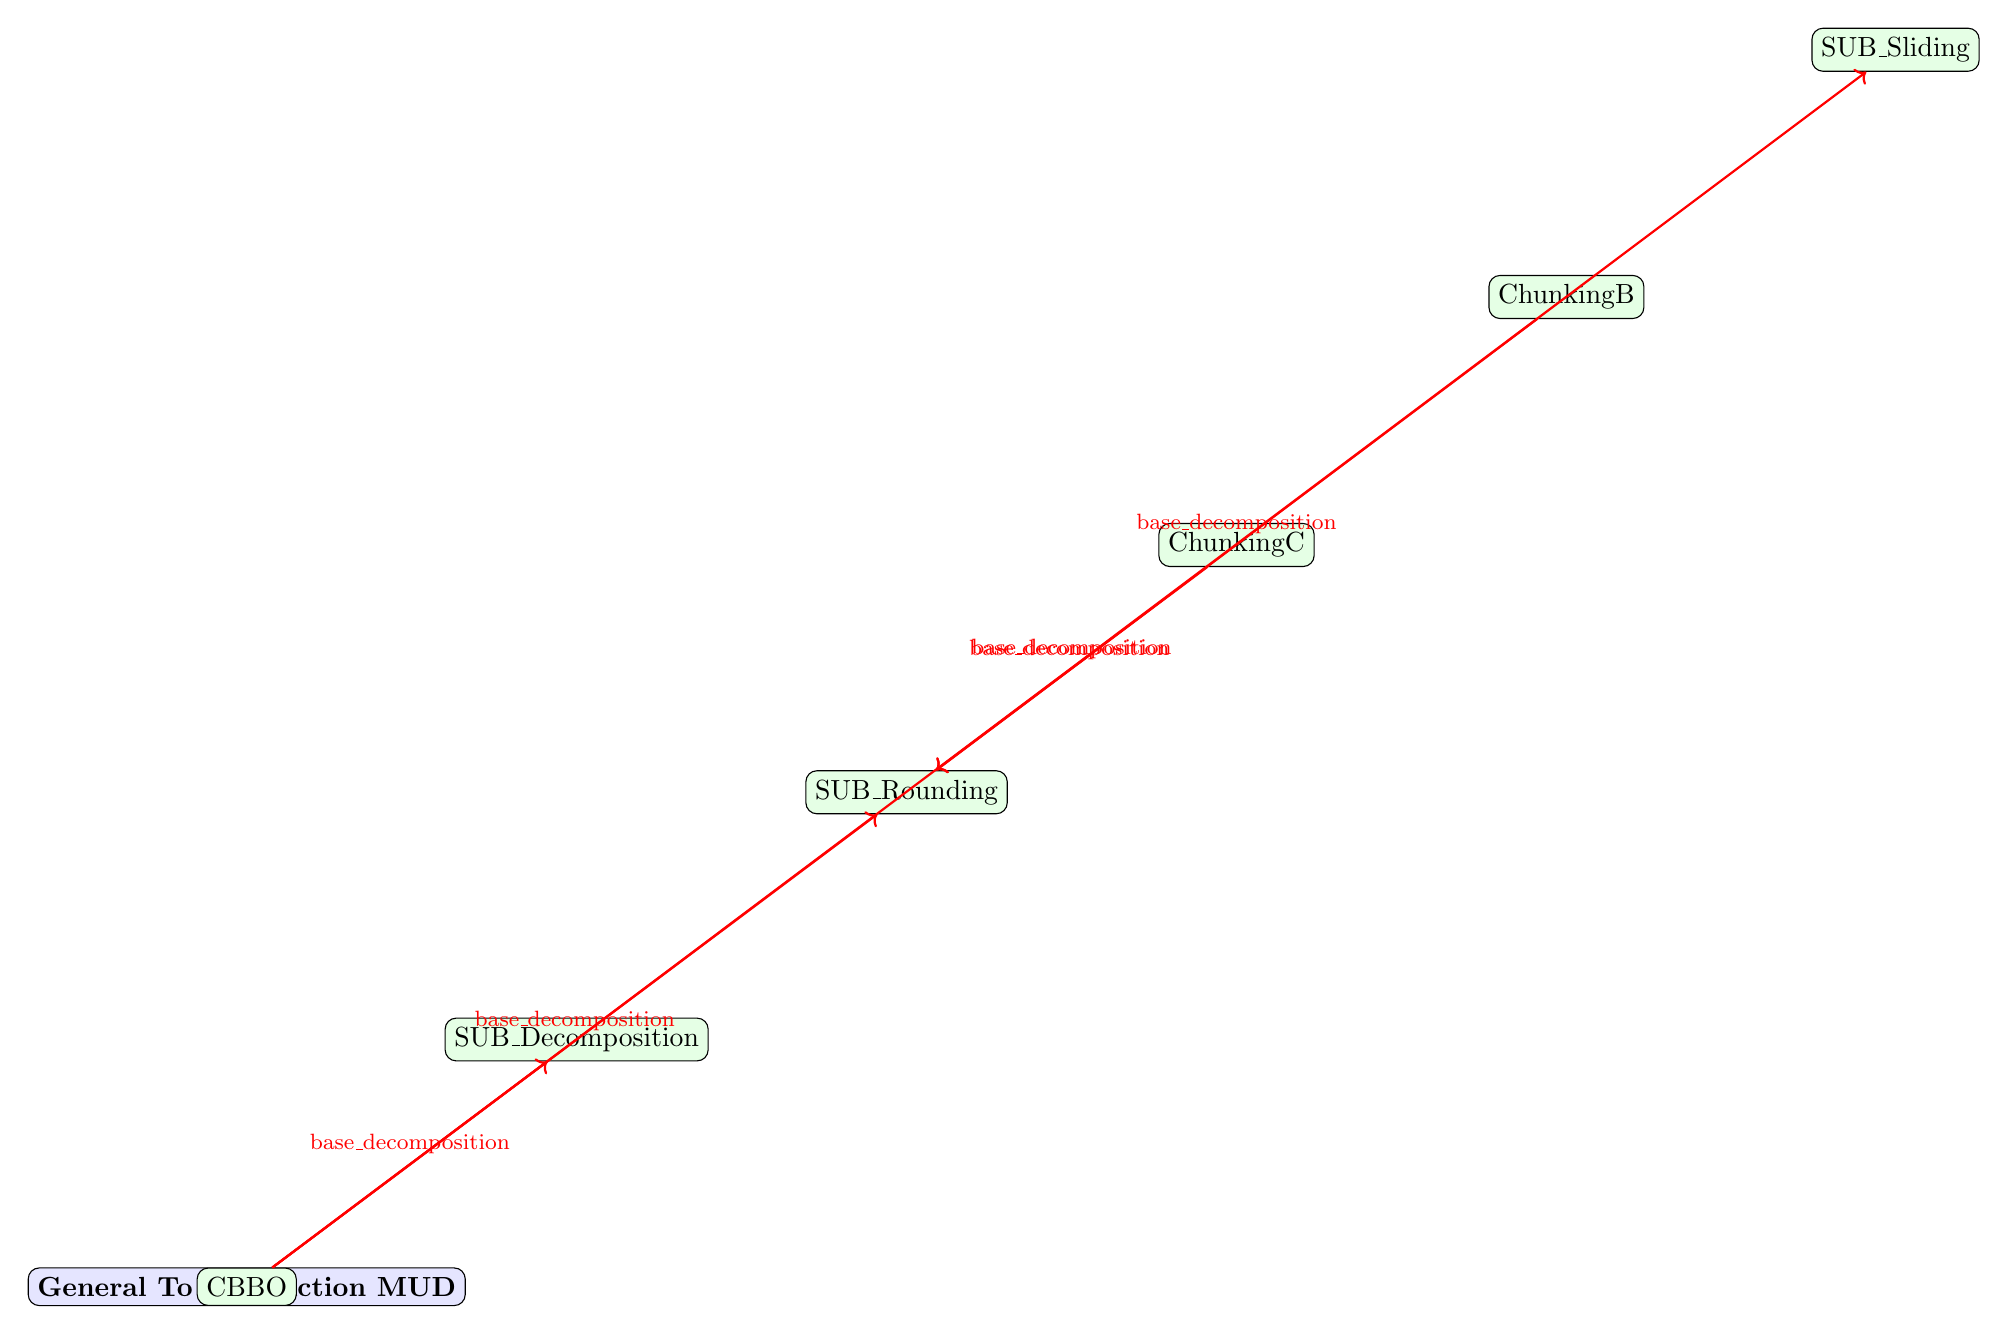
\begin{tikzpicture}[node distance=2cm and 2cm, auto]
\node[draw, fill=blue!10, rounded corners] (title) at (0,0) {\textbf{General To Subtraction MUD}};

\node[draw, fill=green!10, rounded corners] (strategy_0) at (0.00,0.00) {CBBO};
\node[draw, fill=green!10, rounded corners] (strategy_1) at (4.19,3.14) {SUB\_Decomposition};
\node[draw, fill=green!10, rounded corners] (strategy_2) at (8.38,6.28) {SUB\_Rounding};
\node[draw, fill=green!10, rounded corners] (strategy_3) at (12.57,9.42) {ChunkingC};
\node[draw, fill=green!10, rounded corners] (strategy_4) at (16.76,12.57) {ChunkingB};
\node[draw, fill=green!10, rounded corners] (strategy_5) at (20.94,15.71) {SUB\_Sliding};

\draw[red, ->, thick] (strategy_0) -- (strategy_5)
    node[midway, above, font=\footnotesize] {base\_decomposition};
\draw[red, ->, thick] (strategy_0) -- (strategy_1)
    node[midway, above, font=\footnotesize] {base\_decomposition};
\draw[red, ->, thick] (strategy_0) -- (strategy_2)
    node[midway, above, font=\footnotesize] {base\_decomposition};
\draw[red, ->, thick] (strategy_3) -- (strategy_2)
    node[midway, above, font=\footnotesize] {base\_decomposition};
\draw[red, ->, thick] (strategy_4) -- (strategy_2)
    node[midway, above, font=\footnotesize] {base\_decomposition};

\end{tikzpicture}
\end{center}

\textbf{Summary:}\\
\begin{verbatim}
Automated MUD Analysis for General To Subtraction
============================================================
Total strategies analyzed: 6
Total elaborations detected: 5

Key Patterns Identified:
  • base_decomposition: 5 relationships

Notable Elaborations:
  • CBBO → SUB_Sliding
    Shared: base_decomposition (confidence: 1.00)
  • CBBO → SUB_Decomposition
    Shared: base_decomposition (confidence: 1.00)
  • CBBO → SUB_Rounding
    Shared: base_decomposition (confidence: 1.00)
  • ChunkingC → SUB_Rounding
    Shared: base_decomposition (confidence: 1.00)
  • ChunkingB → SUB_Rounding
    Shared: base_decomposition (confidence: 1.00)
\end{verbatim}

\newpage
\subsection{General}

\textbf{Operation:} General\\
\textbf{Strategies Analyzed:} 3\\
\textbf{Elaborations Detected:} 3\\

\begin{center}
\begin{tikzpicture}[node distance=2cm and 2cm, auto]
\node[draw, fill=blue!10, rounded corners] (title) at (0,0) {\textbf{General MUD}};

\node[draw, fill=green!10, rounded corners] (strategy_0) at (0.00,0.00) {CBBO};
\node[draw, fill=green!10, rounded corners] (strategy_1) at (8.38,6.28) {ChunkingC};
\node[draw, fill=green!10, rounded corners] (strategy_2) at (16.76,12.57) {ChunkingB};

\draw[red, ->, thick] (strategy_0) -- (strategy_1)
    node[midway, above, font=\footnotesize] {base\_decomposition};
\draw[red, ->, thick] (strategy_0) -- (strategy_2)
    node[midway, above, font=\footnotesize] {base\_decomposition};
\draw[red, ->, thick] (strategy_1) -- (strategy_2)
    node[midway, above, font=\footnotesize] {base\_decomposition};

\end{tikzpicture}
\end{center}

\textbf{Summary:}\\
\begin{verbatim}
Automated MUD Analysis for General
============================================================
Total strategies analyzed: 3
Total elaborations detected: 3

Key Patterns Identified:
  • base_decomposition: 3 relationships

Notable Elaborations:
  • CBBO → ChunkingC
    Shared: base_decomposition (confidence: 1.00)
  • CBBO → ChunkingB
    Shared: base_decomposition (confidence: 1.00)
  • ChunkingC → ChunkingB
    Shared: base_decomposition (confidence: 1.00)
\end{verbatim}

\newpage
\subsection{General To Multiplication}

\textbf{Operation:} General To Multiplication\\
\textbf{Strategies Analyzed:} 6\\
\textbf{Elaborations Detected:} 4\\

\begin{center}
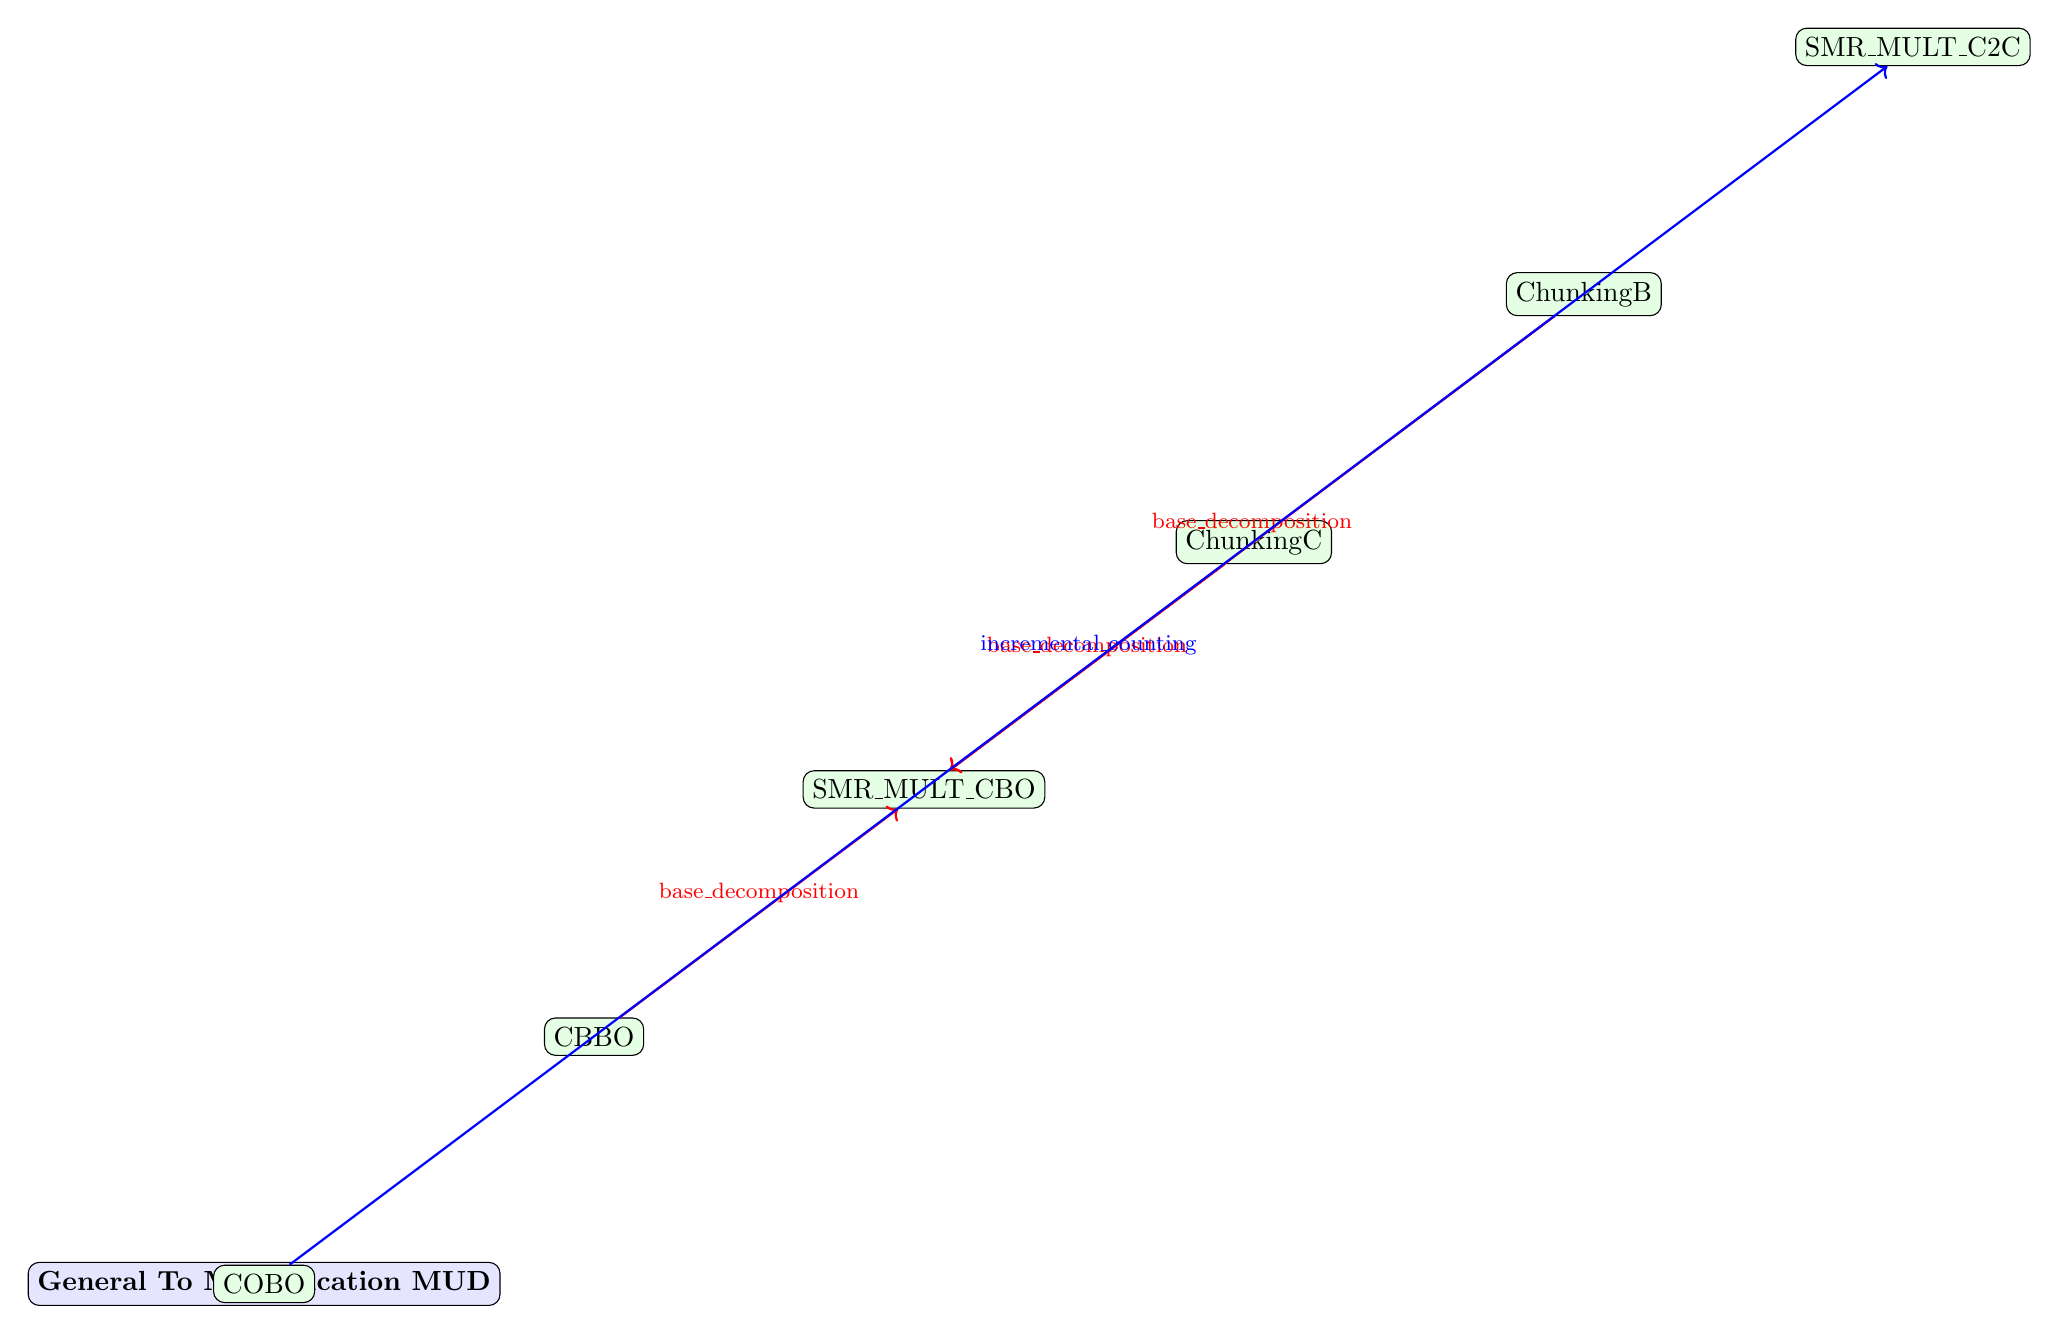
\begin{tikzpicture}[node distance=2cm and 2cm, auto]
\node[draw, fill=blue!10, rounded corners] (title) at (0,0) {\textbf{General To Multiplication MUD}};

\node[draw, fill=green!10, rounded corners] (strategy_0) at (0.00,0.00) {COBO};
\node[draw, fill=green!10, rounded corners] (strategy_1) at (4.19,3.14) {CBBO};
\node[draw, fill=green!10, rounded corners] (strategy_2) at (8.38,6.28) {SMR\_MULT\_CBO};
\node[draw, fill=green!10, rounded corners] (strategy_3) at (12.57,9.42) {ChunkingC};
\node[draw, fill=green!10, rounded corners] (strategy_4) at (16.76,12.57) {ChunkingB};
\node[draw, fill=green!10, rounded corners] (strategy_5) at (20.94,15.71) {SMR\_MULT\_C2C};

\draw[red, ->, thick] (strategy_1) -- (strategy_2)
    node[midway, above, font=\footnotesize] {base\_decomposition};
\draw[red, ->, thick] (strategy_3) -- (strategy_2)
    node[midway, above, font=\footnotesize] {base\_decomposition};
\draw[red, ->, thick] (strategy_4) -- (strategy_2)
    node[midway, above, font=\footnotesize] {base\_decomposition};
\draw[blue, ->, thick] (strategy_0) -- (strategy_5)
    node[midway, above, font=\footnotesize] {incremental\_counting};

\end{tikzpicture}
\end{center}

\textbf{Summary:}\\
\begin{verbatim}
Automated MUD Analysis for General To Multiplication
============================================================
Total strategies analyzed: 6
Total elaborations detected: 4

Key Patterns Identified:
  • base_decomposition: 3 relationships
  • incremental_counting: 1 relationships

Notable Elaborations:
  • CBBO → SMR_MULT_CBO
    Shared: base_decomposition (confidence: 1.00)
  • COBO → SMR_MULT_C2C
    Shared: incremental_counting (confidence: 1.00)
  • ChunkingC → SMR_MULT_CBO
    Shared: base_decomposition (confidence: 1.00)
  • ChunkingB → SMR_MULT_CBO
    Shared: base_decomposition (confidence: 1.00)
\end{verbatim}

\newpage
\subsection{General To Division}

\textbf{Operation:} General To Division\\
\textbf{Strategies Analyzed:} 5\\
\textbf{Elaborations Detected:} 6\\

\begin{center}
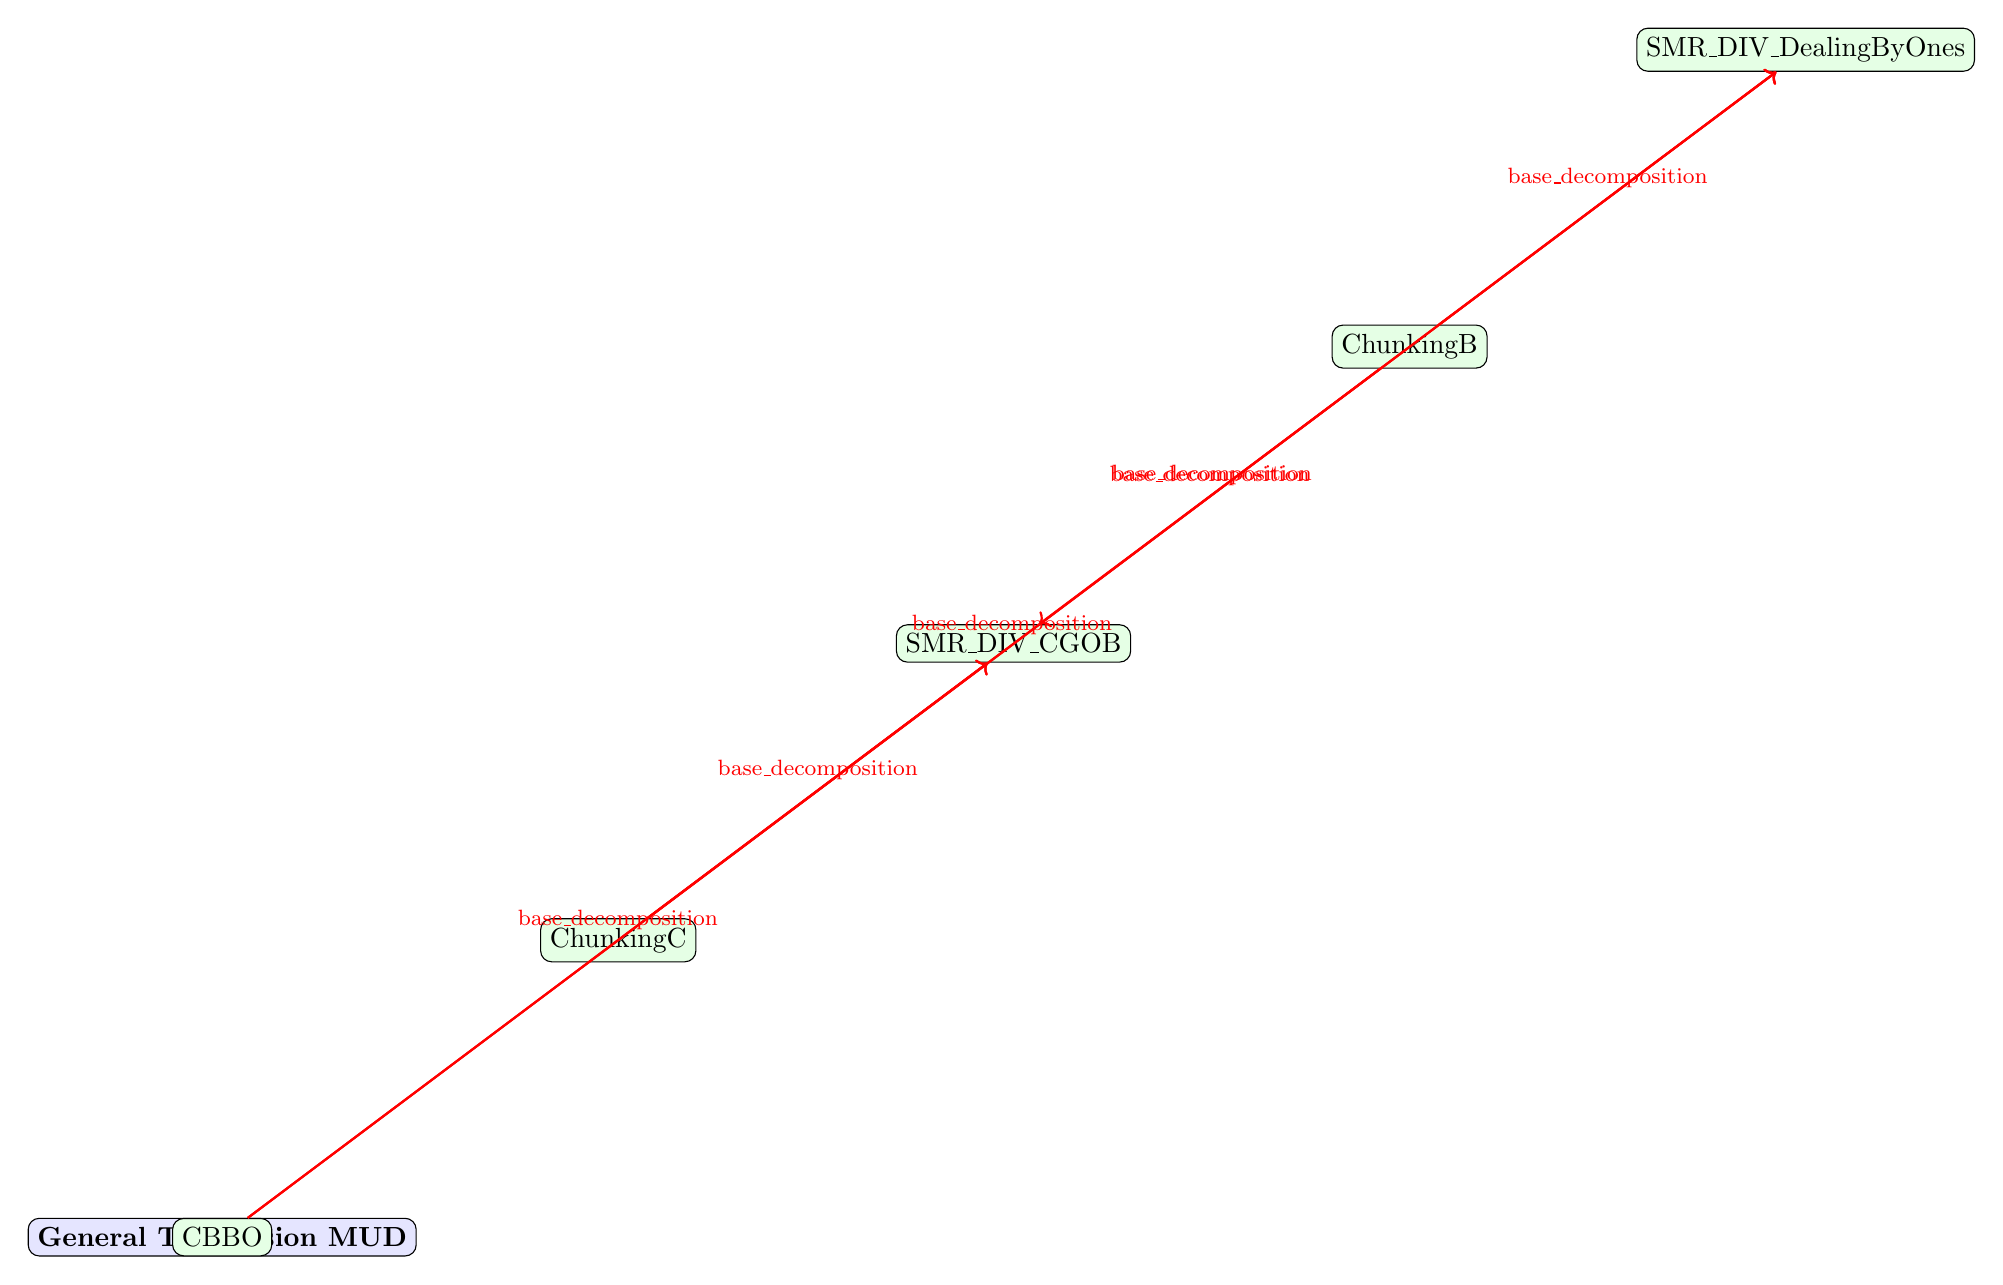
\begin{tikzpicture}[node distance=2cm and 2cm, auto]
\node[draw, fill=blue!10, rounded corners] (title) at (0,0) {\textbf{General To Division MUD}};

\node[draw, fill=green!10, rounded corners] (strategy_0) at (0.00,0.00) {CBBO};
\node[draw, fill=green!10, rounded corners] (strategy_1) at (5.03,3.77) {ChunkingC};
\node[draw, fill=green!10, rounded corners] (strategy_2) at (10.05,7.54) {SMR\_DIV\_CGOB};
\node[draw, fill=green!10, rounded corners] (strategy_3) at (15.08,11.31) {ChunkingB};
\node[draw, fill=green!10, rounded corners] (strategy_4) at (20.11,15.08) {SMR\_DIV\_DealingByOnes};

\draw[red, ->, thick] (strategy_0) -- (strategy_2)
    node[midway, above, font=\footnotesize] {base\_decomposition};
\draw[red, ->, thick] (strategy_0) -- (strategy_4)
    node[midway, above, font=\footnotesize] {base\_decomposition};
\draw[red, ->, thick] (strategy_1) -- (strategy_2)
    node[midway, above, font=\footnotesize] {base\_decomposition};
\draw[red, ->, thick] (strategy_1) -- (strategy_4)
    node[midway, above, font=\footnotesize] {base\_decomposition};
\draw[red, ->, thick] (strategy_3) -- (strategy_2)
    node[midway, above, font=\footnotesize] {base\_decomposition};
\draw[red, ->, thick] (strategy_3) -- (strategy_4)
    node[midway, above, font=\footnotesize] {base\_decomposition};

\end{tikzpicture}
\end{center}

\textbf{Summary:}\\
\begin{verbatim}
Automated MUD Analysis for General To Division
============================================================
Total strategies analyzed: 5
Total elaborations detected: 6

Key Patterns Identified:
  • base_decomposition: 6 relationships

Notable Elaborations:
  • CBBO → SMR_DIV_CGOB
    Shared: base_decomposition (confidence: 1.00)
  • CBBO → SMR_DIV_DealingByOnes
    Shared: base_decomposition (confidence: 1.00)
  • ChunkingC → SMR_DIV_CGOB
    Shared: base_decomposition (confidence: 1.00)
  • ChunkingC → SMR_DIV_DealingByOnes
    Shared: base_decomposition (confidence: 1.00)
  • ChunkingB → SMR_DIV_CGOB
    Shared: base_decomposition (confidence: 1.00)
  ... and 1 more high-confidence relationships
\end{verbatim}

\newpage
\subsection{Subtraction To Addition}

\textbf{Operation:} Subtraction To Addition\\
\textbf{Strategies Analyzed:} 5\\
\textbf{Elaborations Detected:} 6\\

\begin{center}
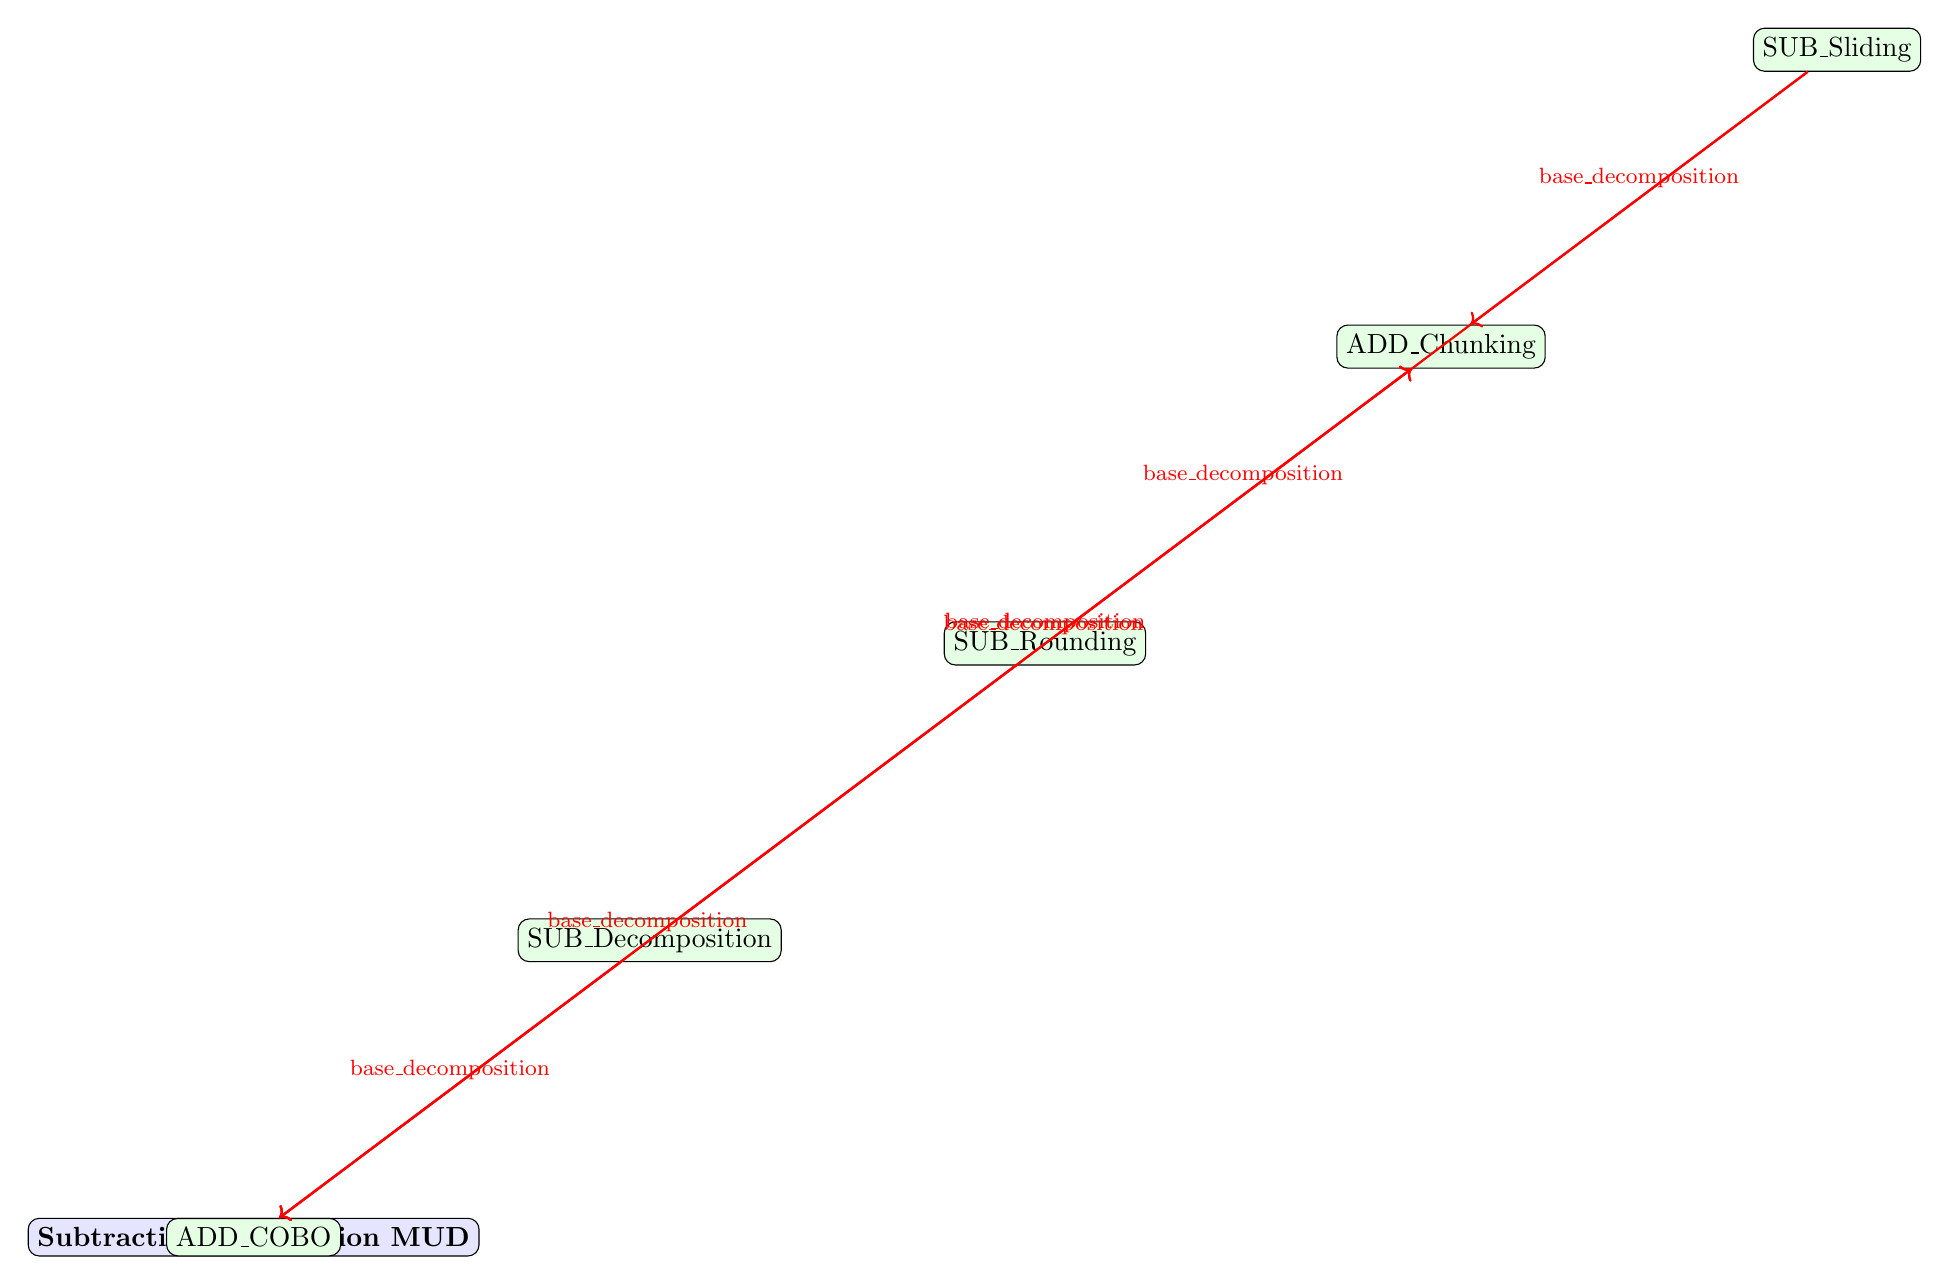
\begin{tikzpicture}[node distance=2cm and 2cm, auto]
\node[draw, fill=blue!10, rounded corners] (title) at (0,0) {\textbf{Subtraction To Addition MUD}};

\node[draw, fill=green!10, rounded corners] (strategy_0) at (0.00,0.00) {ADD\_COBO};
\node[draw, fill=green!10, rounded corners] (strategy_1) at (5.03,3.77) {SUB\_Decomposition};
\node[draw, fill=green!10, rounded corners] (strategy_2) at (10.05,7.54) {SUB\_Rounding};
\node[draw, fill=green!10, rounded corners] (strategy_3) at (15.08,11.31) {ADD\_Chunking};
\node[draw, fill=green!10, rounded corners] (strategy_4) at (20.11,15.08) {SUB\_Sliding};

\draw[red, ->, thick] (strategy_4) -- (strategy_3)
    node[midway, above, font=\footnotesize] {base\_decomposition};
\draw[red, ->, thick] (strategy_1) -- (strategy_3)
    node[midway, above, font=\footnotesize] {base\_decomposition};
\draw[red, ->, thick] (strategy_2) -- (strategy_3)
    node[midway, above, font=\footnotesize] {base\_decomposition};
\draw[red, ->, thick] (strategy_4) -- (strategy_0)
    node[midway, above, font=\footnotesize] {base\_decomposition};
\draw[red, ->, thick] (strategy_1) -- (strategy_0)
    node[midway, above, font=\footnotesize] {base\_decomposition};
\draw[red, ->, thick] (strategy_2) -- (strategy_0)
    node[midway, above, font=\footnotesize] {base\_decomposition};

\end{tikzpicture}
\end{center}

\textbf{Summary:}\\
\begin{verbatim}
Automated MUD Analysis for Subtraction To Addition
============================================================
Total strategies analyzed: 5
Total elaborations detected: 6

Key Patterns Identified:
  • base_decomposition: 6 relationships

Notable Elaborations:
\end{verbatim}

\newpage
\subsection{Multiplication To Addition}

\textbf{Operation:} Multiplication To Addition\\
\textbf{Strategies Analyzed:} 4\\
\textbf{Elaborations Detected:} 4\\

\begin{center}
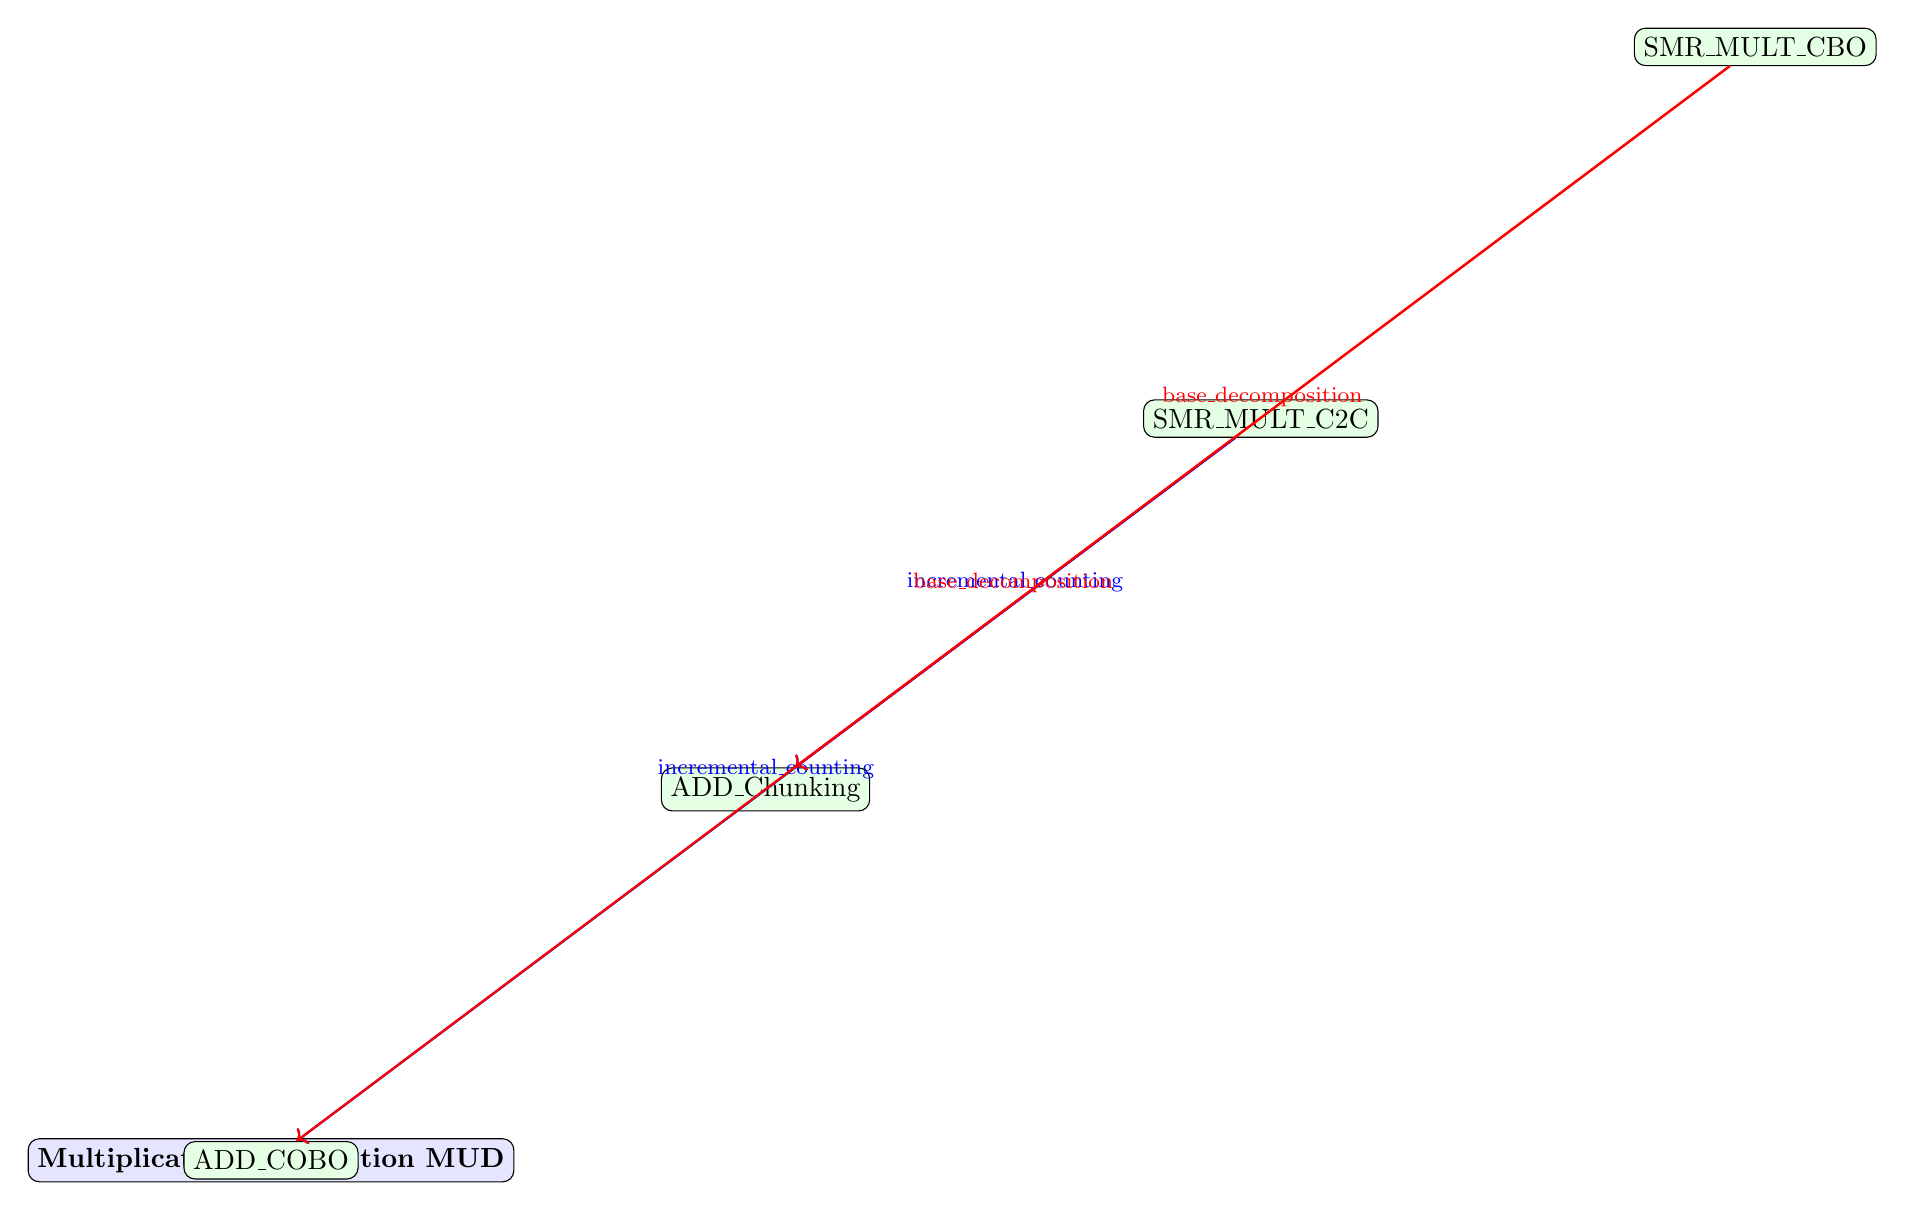
\begin{tikzpicture}[node distance=2cm and 2cm, auto]
\node[draw, fill=blue!10, rounded corners] (title) at (0,0) {\textbf{Multiplication To Addition MUD}};

\node[draw, fill=green!10, rounded corners] (strategy_0) at (0.00,0.00) {ADD\_COBO};
\node[draw, fill=green!10, rounded corners] (strategy_1) at (6.28,4.71) {ADD\_Chunking};
\node[draw, fill=green!10, rounded corners] (strategy_2) at (12.57,9.42) {SMR\_MULT\_C2C};
\node[draw, fill=green!10, rounded corners] (strategy_3) at (18.85,14.14) {SMR\_MULT\_CBO};

\draw[blue, ->, thick] (strategy_2) -- (strategy_1)
    node[midway, above, font=\footnotesize] {incremental\_counting};
\draw[blue, ->, thick] (strategy_2) -- (strategy_0)
    node[midway, above, font=\footnotesize] {incremental\_counting};
\draw[red, ->, thick] (strategy_3) -- (strategy_1)
    node[midway, above, font=\footnotesize] {base\_decomposition};
\draw[red, ->, thick] (strategy_3) -- (strategy_0)
    node[midway, above, font=\footnotesize] {base\_decomposition};

\end{tikzpicture}
\end{center}

\textbf{Summary:}\\
\begin{verbatim}
Automated MUD Analysis for Multiplication To Addition
============================================================
Total strategies analyzed: 4
Total elaborations detected: 4

Key Patterns Identified:
  • incremental_counting: 2 relationships
  • base_decomposition: 2 relationships

Notable Elaborations:
\end{verbatim}

\newpage
\subsection{Division To Addition}

\textbf{Operation:} Division To Addition\\
\textbf{Strategies Analyzed:} 4\\
\textbf{Elaborations Detected:} 4\\

\begin{center}
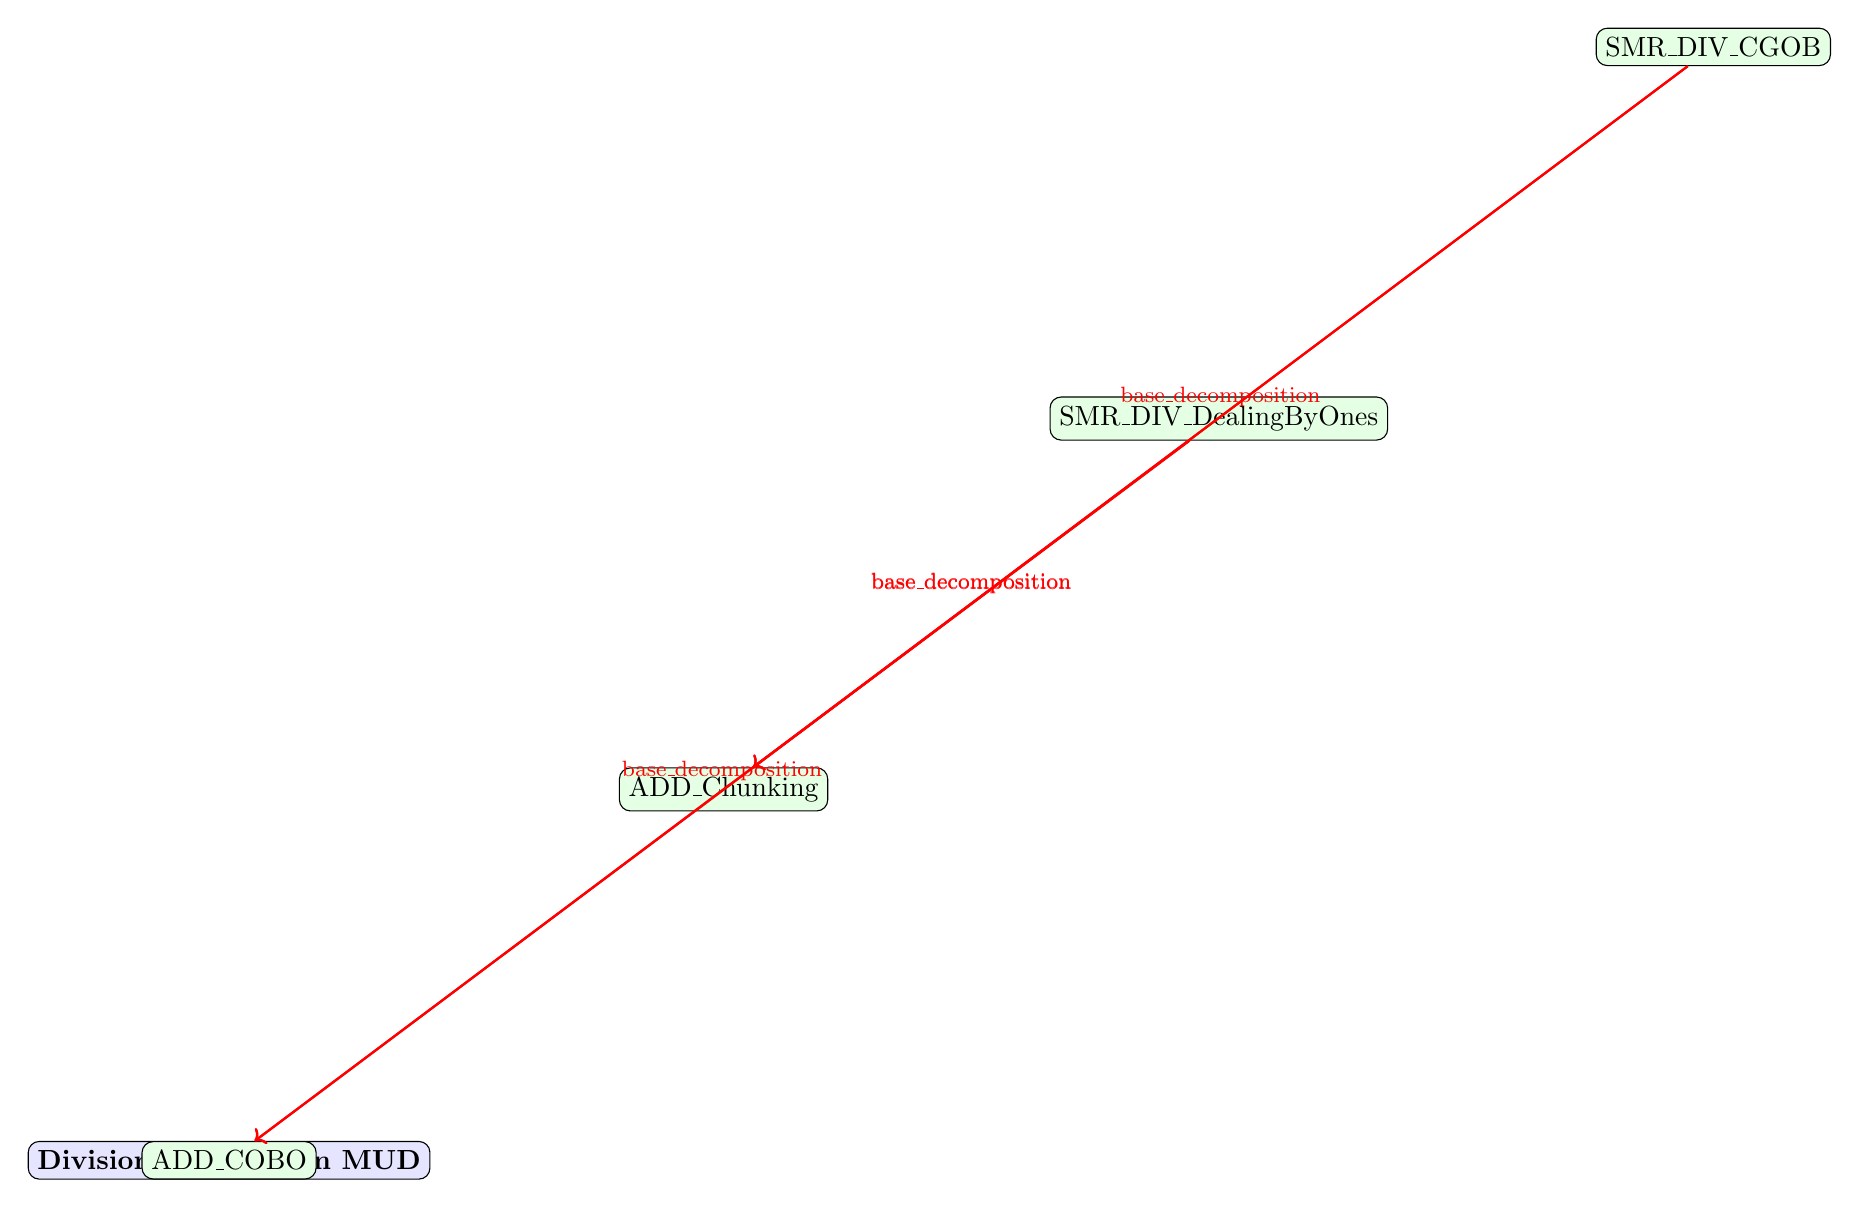
\begin{tikzpicture}[node distance=2cm and 2cm, auto]
\node[draw, fill=blue!10, rounded corners] (title) at (0,0) {\textbf{Division To Addition MUD}};

\node[draw, fill=green!10, rounded corners] (strategy_0) at (0.00,0.00) {ADD\_COBO};
\node[draw, fill=green!10, rounded corners] (strategy_1) at (6.28,4.71) {ADD\_Chunking};
\node[draw, fill=green!10, rounded corners] (strategy_2) at (12.57,9.42) {SMR\_DIV\_DealingByOnes};
\node[draw, fill=green!10, rounded corners] (strategy_3) at (18.85,14.14) {SMR\_DIV\_CGOB};

\draw[red, ->, thick] (strategy_3) -- (strategy_1)
    node[midway, above, font=\footnotesize] {base\_decomposition};
\draw[red, ->, thick] (strategy_2) -- (strategy_1)
    node[midway, above, font=\footnotesize] {base\_decomposition};
\draw[red, ->, thick] (strategy_3) -- (strategy_0)
    node[midway, above, font=\footnotesize] {base\_decomposition};
\draw[red, ->, thick] (strategy_2) -- (strategy_0)
    node[midway, above, font=\footnotesize] {base\_decomposition};

\end{tikzpicture}
\end{center}

\textbf{Summary:}\\
\begin{verbatim}
Automated MUD Analysis for Division To Addition
============================================================
Total strategies analyzed: 4
Total elaborations detected: 4

Key Patterns Identified:
  • base_decomposition: 4 relationships

Notable Elaborations:
\end{verbatim}

\newpage
\subsection{Subtraction}

\textbf{Operation:} Subtraction\\
\textbf{Strategies Analyzed:} 3\\
\textbf{Elaborations Detected:} 3\\

\begin{center}
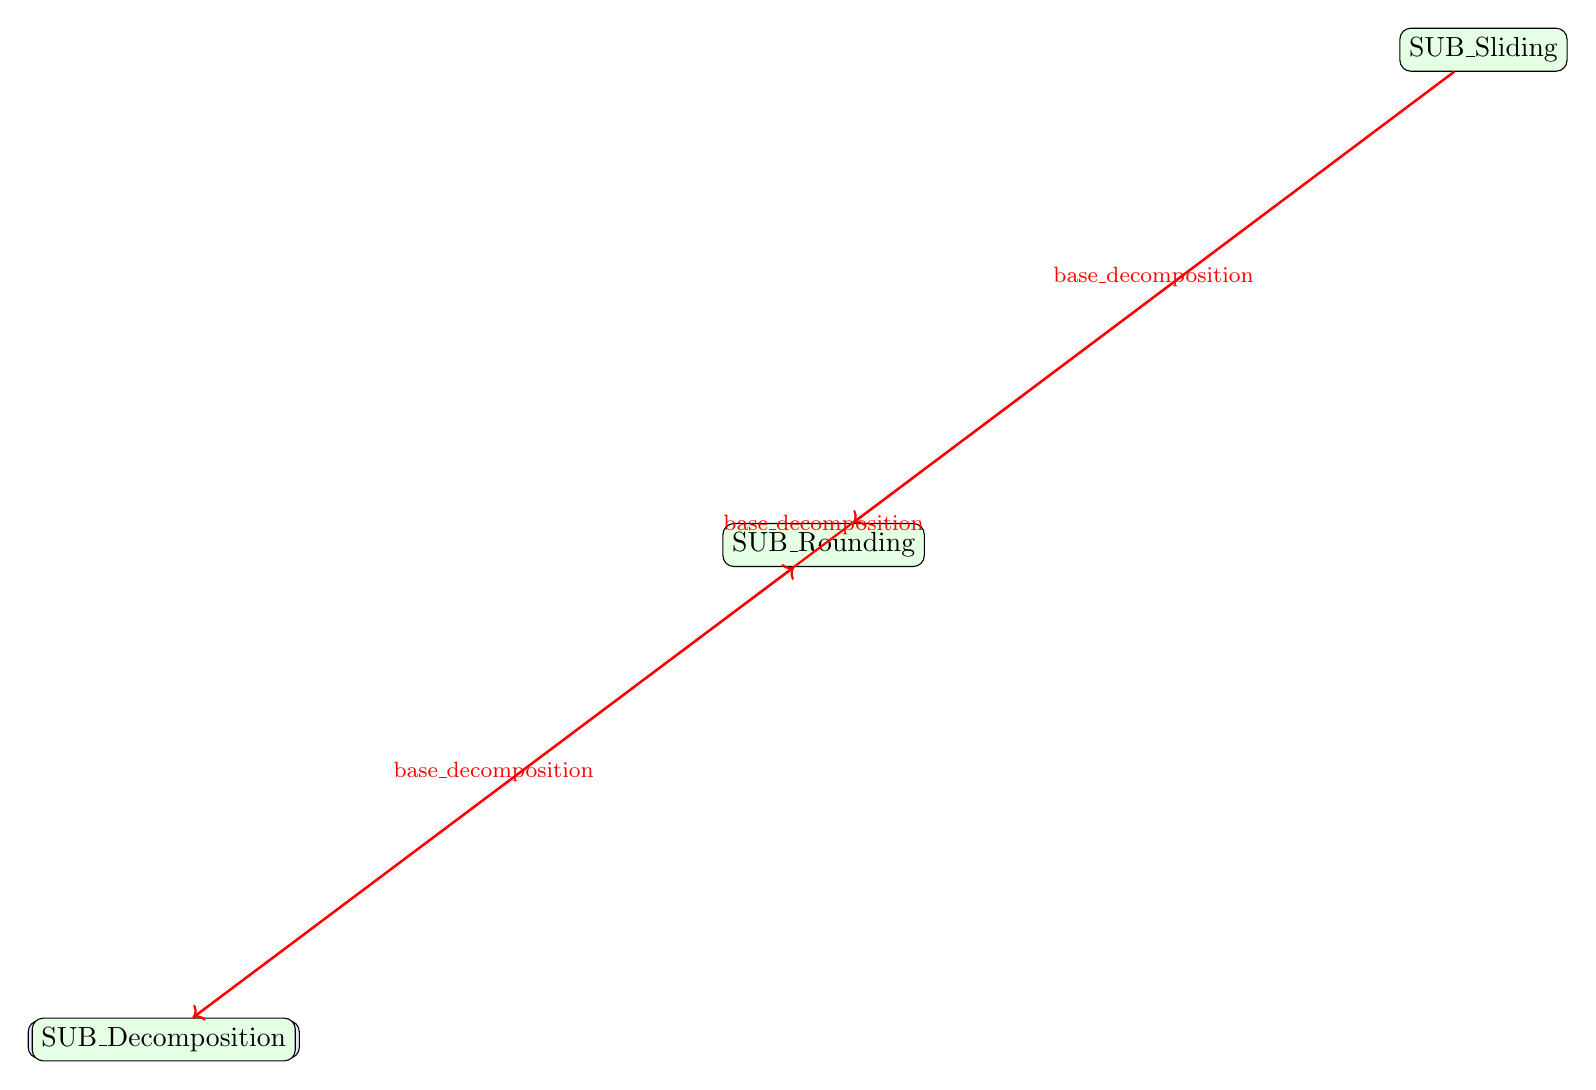
\begin{tikzpicture}[node distance=2cm and 2cm, auto]
\node[draw, fill=blue!10, rounded corners] (title) at (0,0) {\textbf{Subtraction MUD}};

\node[draw, fill=green!10, rounded corners] (strategy_0) at (0.00,0.00) {SUB\_Decomposition};
\node[draw, fill=green!10, rounded corners] (strategy_1) at (8.38,6.28) {SUB\_Rounding};
\node[draw, fill=green!10, rounded corners] (strategy_2) at (16.76,12.57) {SUB\_Sliding};

\draw[red, ->, thick] (strategy_2) -- (strategy_0)
    node[midway, above, font=\footnotesize] {base\_decomposition};
\draw[red, ->, thick] (strategy_2) -- (strategy_1)
    node[midway, above, font=\footnotesize] {base\_decomposition};
\draw[red, ->, thick] (strategy_0) -- (strategy_1)
    node[midway, above, font=\footnotesize] {base\_decomposition};

\end{tikzpicture}
\end{center}

\textbf{Summary:}\\
\begin{verbatim}
Automated MUD Analysis for Subtraction
============================================================
Total strategies analyzed: 3
Total elaborations detected: 3

Key Patterns Identified:
  • base_decomposition: 3 relationships

Notable Elaborations:
  • SUB_Sliding → SUB_Decomposition
    Shared: base_decomposition (confidence: 1.00)
  • SUB_Sliding → SUB_Rounding
    Shared: base_decomposition (confidence: 1.00)
  • SUB_Decomposition → SUB_Rounding
    Shared: base_decomposition (confidence: 1.00)
\end{verbatim}

\newpage
\subsection{Subtraction To General}

\textbf{Operation:} Subtraction To General\\
\textbf{Strategies Analyzed:} 4\\
\textbf{Elaborations Detected:} 4\\

\begin{center}
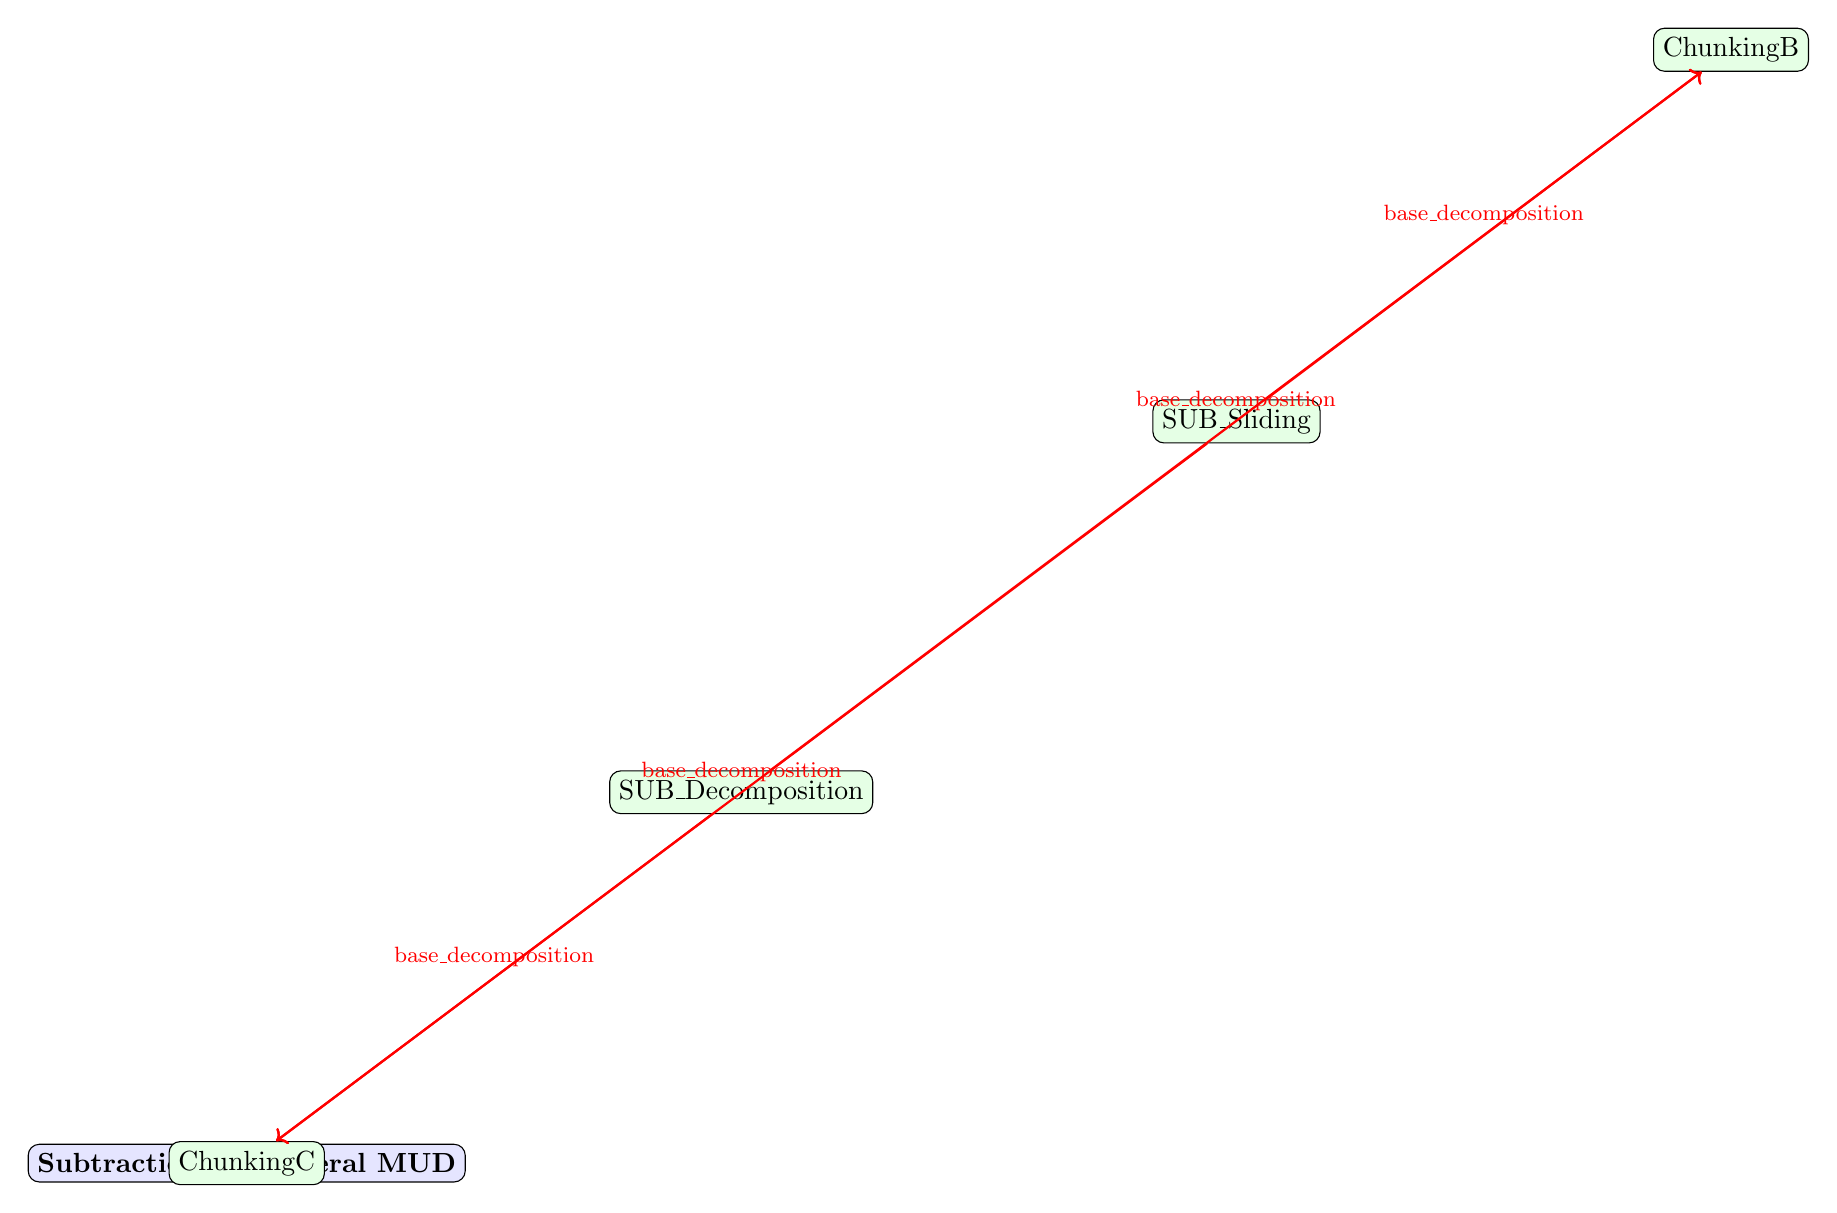
\begin{tikzpicture}[node distance=2cm and 2cm, auto]
\node[draw, fill=blue!10, rounded corners] (title) at (0,0) {\textbf{Subtraction To General MUD}};

\node[draw, fill=green!10, rounded corners] (strategy_0) at (0.00,0.00) {ChunkingC};
\node[draw, fill=green!10, rounded corners] (strategy_1) at (6.28,4.71) {SUB\_Decomposition};
\node[draw, fill=green!10, rounded corners] (strategy_2) at (12.57,9.42) {SUB\_Sliding};
\node[draw, fill=green!10, rounded corners] (strategy_3) at (18.85,14.14) {ChunkingB};

\draw[red, ->, thick] (strategy_2) -- (strategy_0)
    node[midway, above, font=\footnotesize] {base\_decomposition};
\draw[red, ->, thick] (strategy_2) -- (strategy_3)
    node[midway, above, font=\footnotesize] {base\_decomposition};
\draw[red, ->, thick] (strategy_1) -- (strategy_0)
    node[midway, above, font=\footnotesize] {base\_decomposition};
\draw[red, ->, thick] (strategy_1) -- (strategy_3)
    node[midway, above, font=\footnotesize] {base\_decomposition};

\end{tikzpicture}
\end{center}

\textbf{Summary:}\\
\begin{verbatim}
Automated MUD Analysis for Subtraction To General
============================================================
Total strategies analyzed: 4
Total elaborations detected: 4

Key Patterns Identified:
  • base_decomposition: 4 relationships

Notable Elaborations:
  • SUB_Sliding → ChunkingC
    Shared: base_decomposition (confidence: 1.00)
  • SUB_Sliding → ChunkingB
    Shared: base_decomposition (confidence: 1.00)
  • SUB_Decomposition → ChunkingC
    Shared: base_decomposition (confidence: 1.00)
  • SUB_Decomposition → ChunkingB
    Shared: base_decomposition (confidence: 1.00)
\end{verbatim}

\newpage
\subsection{Subtraction To Multiplication}

\textbf{Operation:} Subtraction To Multiplication\\
\textbf{Strategies Analyzed:} 4\\
\textbf{Elaborations Detected:} 3\\

\begin{center}
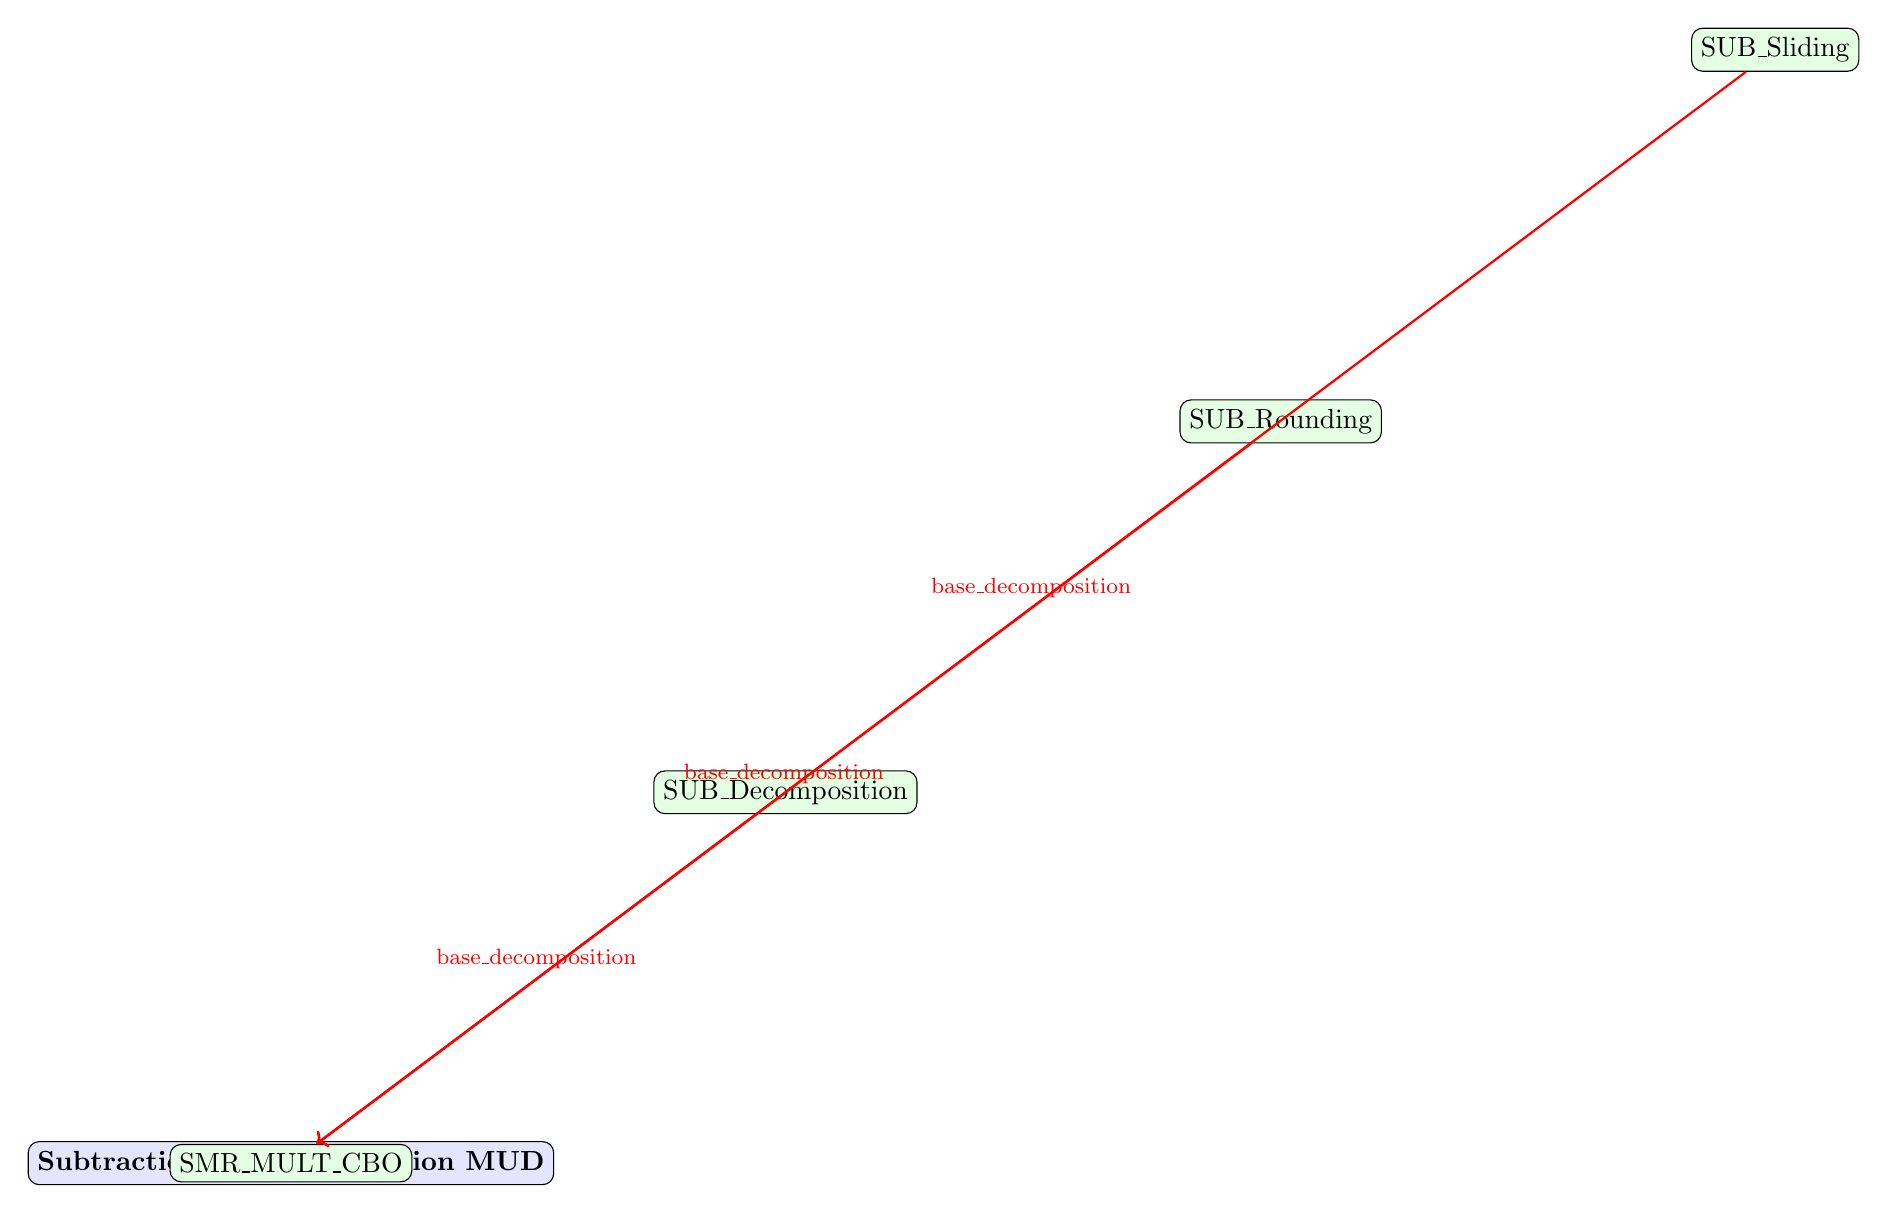
\begin{tikzpicture}[node distance=2cm and 2cm, auto]
\node[draw, fill=blue!10, rounded corners] (title) at (0,0) {\textbf{Subtraction To Multiplication MUD}};

\node[draw, fill=green!10, rounded corners] (strategy_0) at (0.00,0.00) {SMR\_MULT\_CBO};
\node[draw, fill=green!10, rounded corners] (strategy_1) at (6.28,4.71) {SUB\_Decomposition};
\node[draw, fill=green!10, rounded corners] (strategy_2) at (12.57,9.42) {SUB\_Rounding};
\node[draw, fill=green!10, rounded corners] (strategy_3) at (18.85,14.14) {SUB\_Sliding};

\draw[red, ->, thick] (strategy_3) -- (strategy_0)
    node[midway, above, font=\footnotesize] {base\_decomposition};
\draw[red, ->, thick] (strategy_1) -- (strategy_0)
    node[midway, above, font=\footnotesize] {base\_decomposition};
\draw[red, ->, thick] (strategy_2) -- (strategy_0)
    node[midway, above, font=\footnotesize] {base\_decomposition};

\end{tikzpicture}
\end{center}

\textbf{Summary:}\\
\begin{verbatim}
Automated MUD Analysis for Subtraction To Multiplication
============================================================
Total strategies analyzed: 4
Total elaborations detected: 3

Key Patterns Identified:
  • base_decomposition: 3 relationships

Notable Elaborations:
  • SUB_Sliding → SMR_MULT_CBO
    Shared: base_decomposition (confidence: 1.00)
  • SUB_Decomposition → SMR_MULT_CBO
    Shared: base_decomposition (confidence: 1.00)
  • SUB_Rounding → SMR_MULT_CBO
    Shared: base_decomposition (confidence: 1.00)
\end{verbatim}

\newpage
\subsection{Subtraction To Division}

\textbf{Operation:} Subtraction To Division\\
\textbf{Strategies Analyzed:} 5\\
\textbf{Elaborations Detected:} 6\\

\begin{center}
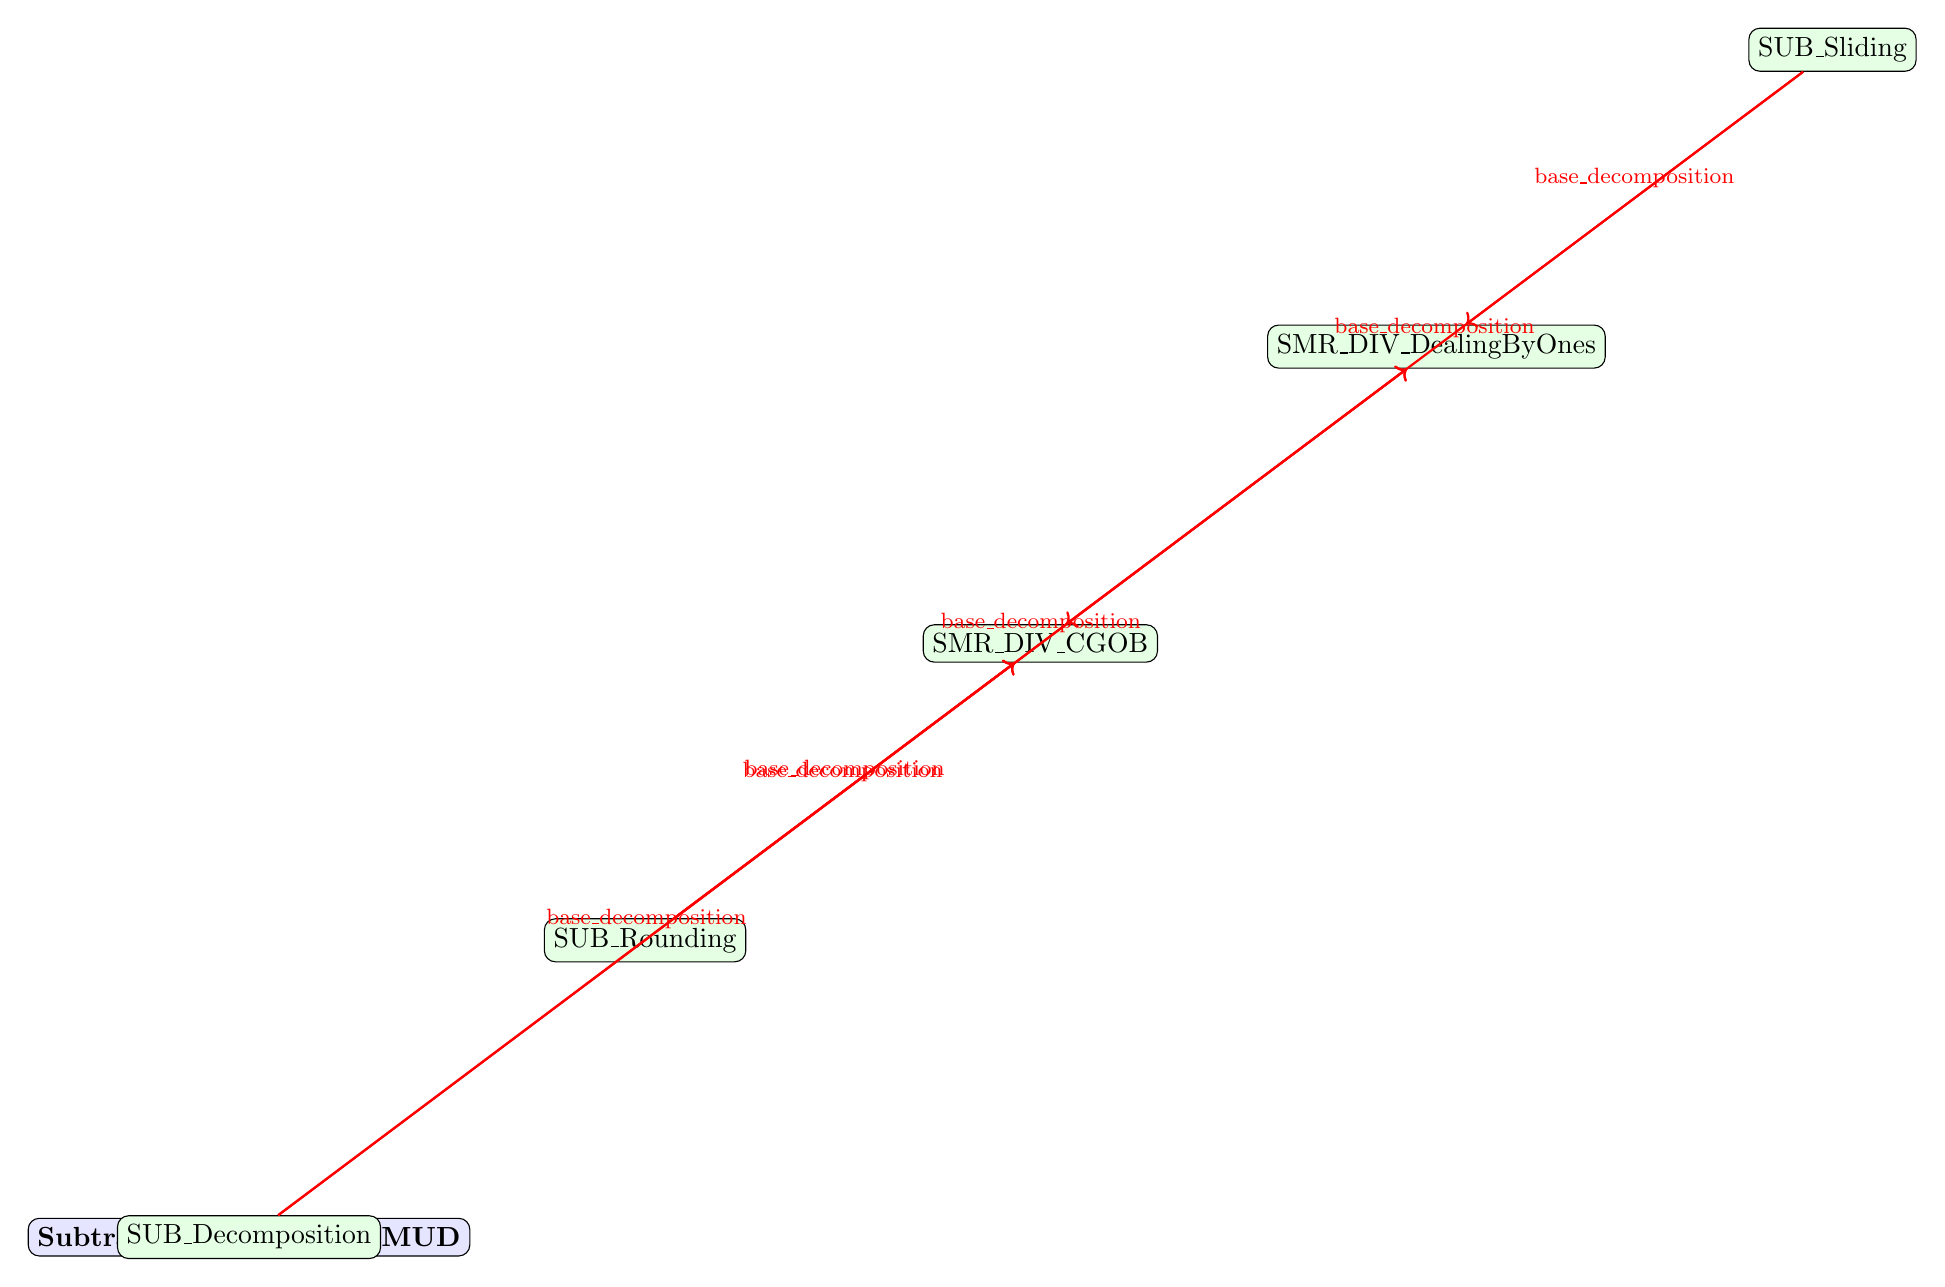
\begin{tikzpicture}[node distance=2cm and 2cm, auto]
\node[draw, fill=blue!10, rounded corners] (title) at (0,0) {\textbf{Subtraction To Division MUD}};

\node[draw, fill=green!10, rounded corners] (strategy_0) at (0.00,0.00) {SUB\_Decomposition};
\node[draw, fill=green!10, rounded corners] (strategy_1) at (5.03,3.77) {SUB\_Rounding};
\node[draw, fill=green!10, rounded corners] (strategy_2) at (10.05,7.54) {SMR\_DIV\_CGOB};
\node[draw, fill=green!10, rounded corners] (strategy_3) at (15.08,11.31) {SMR\_DIV\_DealingByOnes};
\node[draw, fill=green!10, rounded corners] (strategy_4) at (20.11,15.08) {SUB\_Sliding};

\draw[red, ->, thick] (strategy_4) -- (strategy_2)
    node[midway, above, font=\footnotesize] {base\_decomposition};
\draw[red, ->, thick] (strategy_4) -- (strategy_3)
    node[midway, above, font=\footnotesize] {base\_decomposition};
\draw[red, ->, thick] (strategy_0) -- (strategy_2)
    node[midway, above, font=\footnotesize] {base\_decomposition};
\draw[red, ->, thick] (strategy_0) -- (strategy_3)
    node[midway, above, font=\footnotesize] {base\_decomposition};
\draw[red, ->, thick] (strategy_1) -- (strategy_2)
    node[midway, above, font=\footnotesize] {base\_decomposition};
\draw[red, ->, thick] (strategy_1) -- (strategy_3)
    node[midway, above, font=\footnotesize] {base\_decomposition};

\end{tikzpicture}
\end{center}

\textbf{Summary:}\\
\begin{verbatim}
Automated MUD Analysis for Subtraction To Division
============================================================
Total strategies analyzed: 5
Total elaborations detected: 6

Key Patterns Identified:
  • base_decomposition: 6 relationships

Notable Elaborations:
  • SUB_Sliding → SMR_DIV_CGOB
    Shared: base_decomposition (confidence: 1.00)
  • SUB_Sliding → SMR_DIV_DealingByOnes
    Shared: base_decomposition (confidence: 1.00)
  • SUB_Decomposition → SMR_DIV_CGOB
    Shared: base_decomposition (confidence: 1.00)
  • SUB_Decomposition → SMR_DIV_DealingByOnes
    Shared: base_decomposition (confidence: 1.00)
  • SUB_Rounding → SMR_DIV_CGOB
    Shared: base_decomposition (confidence: 1.00)
  ... and 1 more high-confidence relationships
\end{verbatim}

\newpage
\subsection{Multiplication To Division}

\textbf{Operation:} Multiplication To Division\\
\textbf{Strategies Analyzed:} 3\\
\textbf{Elaborations Detected:} 2\\

\begin{center}
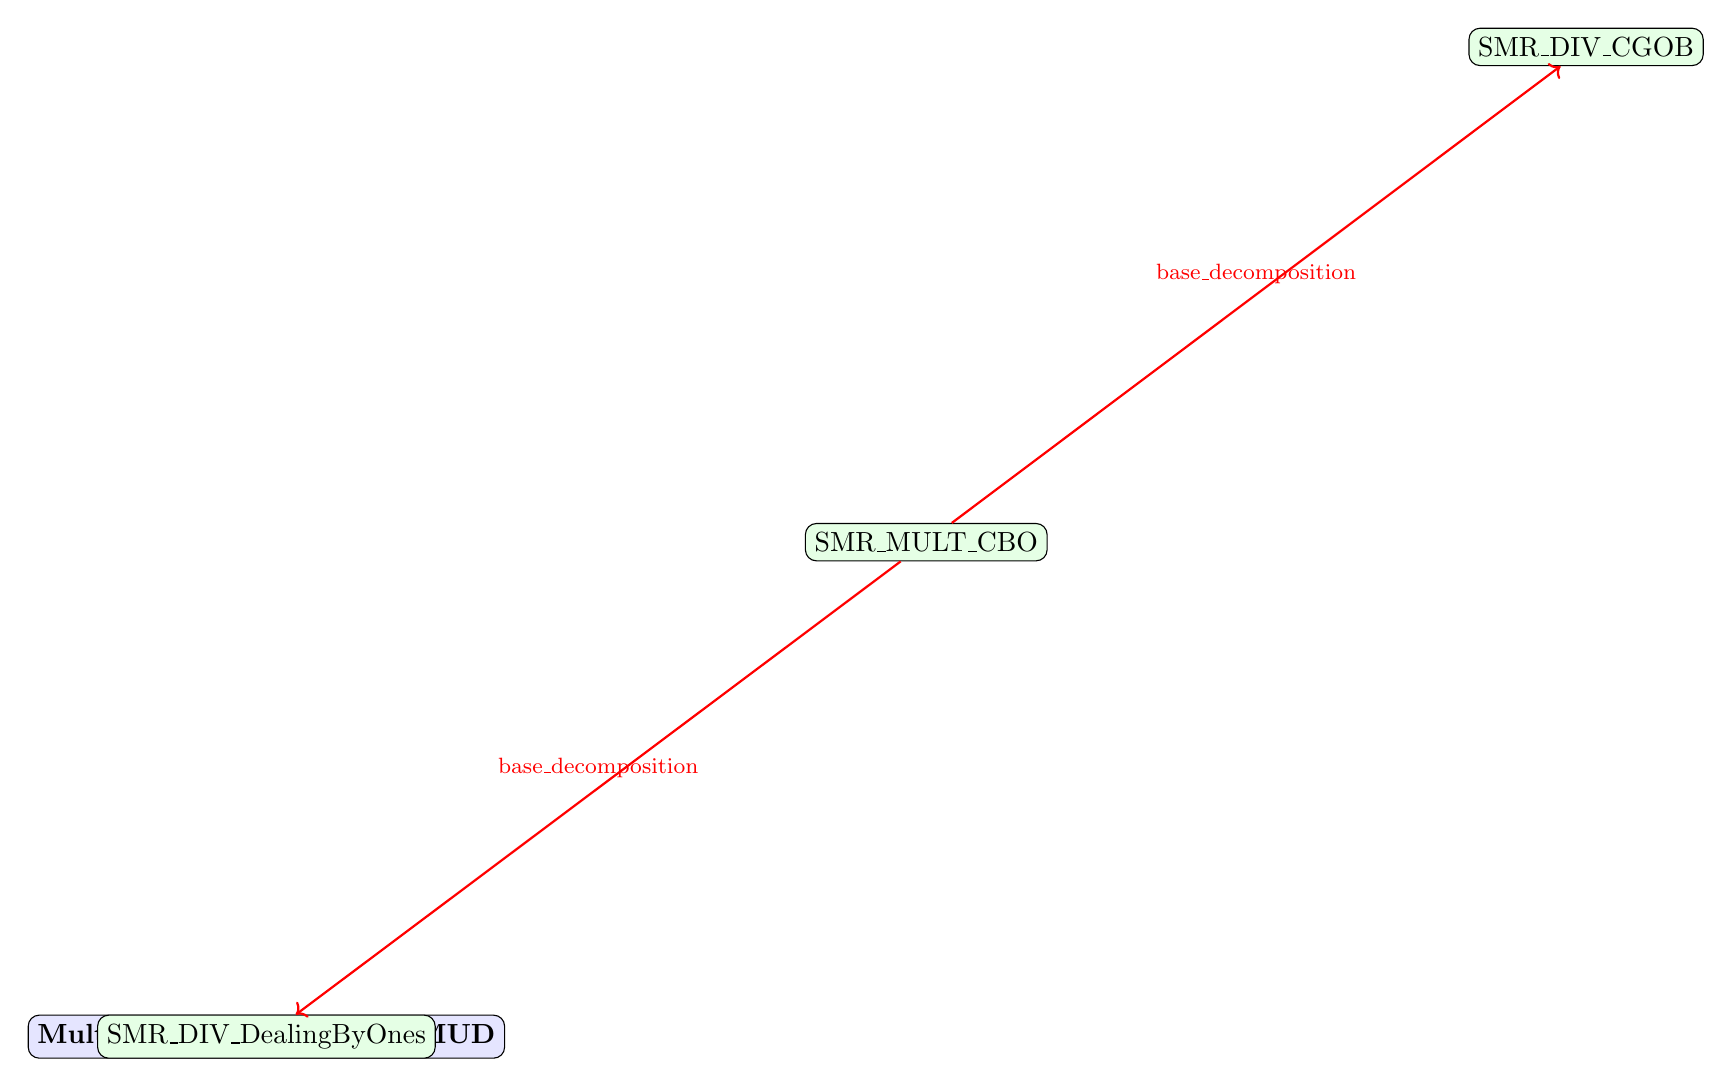
\begin{tikzpicture}[node distance=2cm and 2cm, auto]
\node[draw, fill=blue!10, rounded corners] (title) at (0,0) {\textbf{Multiplication To Division MUD}};

\node[draw, fill=green!10, rounded corners] (strategy_0) at (0.00,0.00) {SMR\_DIV\_DealingByOnes};
\node[draw, fill=green!10, rounded corners] (strategy_1) at (8.38,6.28) {SMR\_MULT\_CBO};
\node[draw, fill=green!10, rounded corners] (strategy_2) at (16.76,12.57) {SMR\_DIV\_CGOB};

\draw[red, ->, thick] (strategy_1) -- (strategy_2)
    node[midway, above, font=\footnotesize] {base\_decomposition};
\draw[red, ->, thick] (strategy_1) -- (strategy_0)
    node[midway, above, font=\footnotesize] {base\_decomposition};

\end{tikzpicture}
\end{center}

\textbf{Summary:}\\
\begin{verbatim}
Automated MUD Analysis for Multiplication To Division
============================================================
Total strategies analyzed: 3
Total elaborations detected: 2

Key Patterns Identified:
  • base_decomposition: 2 relationships

Notable Elaborations:
  • SMR_MULT_CBO → SMR_DIV_CGOB
    Shared: base_decomposition (confidence: 1.00)
  • SMR_MULT_CBO → SMR_DIV_DealingByOnes
    Shared: base_decomposition (confidence: 1.00)
\end{verbatim}

\newpage
\subsection{Division}

\textbf{Operation:} Division\\
\textbf{Strategies Analyzed:} 2\\
\textbf{Elaborations Detected:} 1\\

\begin{center}
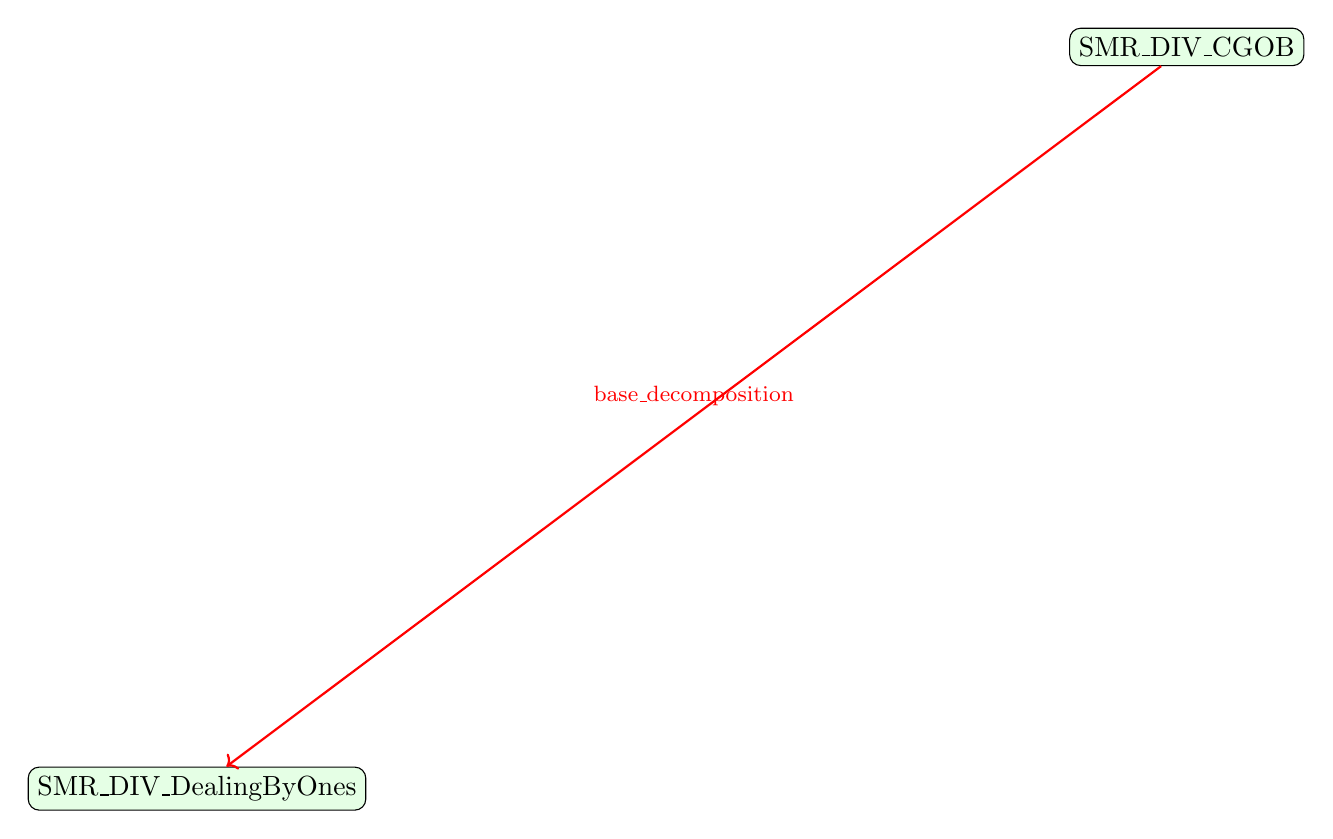
\begin{tikzpicture}[node distance=2cm and 2cm, auto]
\node[draw, fill=blue!10, rounded corners] (title) at (0,0) {\textbf{Division MUD}};

\node[draw, fill=green!10, rounded corners] (strategy_0) at (0.00,0.00) {SMR\_DIV\_DealingByOnes};
\node[draw, fill=green!10, rounded corners] (strategy_1) at (12.57,9.42) {SMR\_DIV\_CGOB};

\draw[red, ->, thick] (strategy_1) -- (strategy_0)
    node[midway, above, font=\footnotesize] {base\_decomposition};

\end{tikzpicture}
\end{center}

\textbf{Summary:}\\
\begin{verbatim}
Automated MUD Analysis for Division
============================================================
Total strategies analyzed: 2
Total elaborations detected: 1

Key Patterns Identified:
  • base_decomposition: 1 relationships

Notable Elaborations:
  • SMR_DIV_CGOB → SMR_DIV_DealingByOnes
    Shared: base_decomposition (confidence: 1.00)
\end{verbatim}

\newpage

\end{document}